
\documentclass[xcolor=dvipsnames]{beamer}  % for hardcopy add 'trans'

\mode<presentation>
{
  \usetheme{Singapore}
  % or ...
  \setbeamercovered{transparent}
  % or whatever (possibly just delete it)
}

\usefonttheme{professionalfonts}
\usepackage[russian]{babel}
% or whatever
%\usepackage[latin1]{inputenc}
% or whatever
%\usepackage{times}
%\usepackage[T1]{fontenc}
% Or whatever. Note that the encoding and the font should match. If T1
% does not look nice, try deleting the line with the fontenc.

%%%%%%%%%%%%%%%%%%%%%% start my preamble %%%%%%%%%%%%%%%%%%%%%%


\addtobeamertemplate{navigation symbols}{}{%
    \usebeamerfont{footline}%
    \usebeamercolor[fg]{footline}%
    \hspace{1em}%
    \insertframenumber/\inserttotalframenumber
} 

\setbeamercolor{footline}{fg=blue}
\setbeamerfont{footline}{series=\bfseries}


%\usepackage{epsfig}
\usepackage{graphicx}
\graphicspath{{./figs_code/}}

\usepackage{amsmath, amssymb, amsthm}

\usepackage{fancyvrb}

\usepackage{tikz}
\usetikzlibrary{arrows}
\usetikzlibrary{calc}
\usetikzlibrary{intersections}
\usetikzlibrary{decorations}
\usepackage{pgf}
\usepackage{pgfplots}
\pgfplotsset{compat=1.13}

\usepackage{graphviz}
 
\usepackage{verbatim}


\usepackage{algorithmicx,algpseudocode}


%font
\usepackage{mathpazo}
%\usepackage[usenames, dvipsnames]{color}

%\usepackage[linesnumbered, ruled, lined]{algorithm2e}

\usepackage{xr}
\externaldocument[ET-]{et}


\newcommand*{\theorembreak}{\usebeamertemplate{theorem end}\framebreak\usebeamertemplate{theorem begin}}

\newcommand{\newtopic}[1]{\textcolor{Green}{\Large \bf #1}}
\newcommand{\navy}[1]{\textcolor{Blue}{\bf #1}}
\newcommand{\navymth}[1]{\textcolor{Blue}{#1}}
\newcommand{\red}[1]{\textcolor{red}{#1}}


\definecolor{pale}{RGB}{235, 235, 235}
\definecolor{pale2}{RGB}{175,238,238}
\definecolor{turquois4}{RGB}{0,134,139}

% Typesetting code
\definecolor{bg}{rgb}{0.95,0.95,0.95}
\usepackage{minted}
\usemintedstyle{friendly}
\newminted{python}{mathescape,frame=lines,framesep=4mm,bgcolor=bg}
\newminted{ipython}{mathescape,frame=lines,framesep=4mm,bgcolor=bg}
\newminted{julia}{mathescape,frame=lines,framesep=4mm,bgcolor=bg}
\newminted{c}{mathescape,linenos=true}
\newminted{r}{mathescape,  frame=none, baselinestretch=1, framesep=2mm}
\renewcommand{\theFancyVerbLine}{\sffamily
    \textcolor[rgb]{0.5,0.5,1.0}{\scriptsize {\arabic{FancyVerbLine}}}}


\usepackage{stmaryrd}

\newcommand{\Fact}{\textcolor{Brown}{\bf Факт. }}
\newcommand{\Facts}{\textcolor{Brown}{\bf Факты }}
\newcommand{\keya}{\textcolor{turquois4}{\bf Ключевая идея. }}
\newcommand{\Factnodot}{\textcolor{Brown}{\bf Факт }}
\newcommand{\Eg}{\textcolor{ForestGreen}{Пример. }}
\newcommand{\Egs}{\textcolor{ForestGreen}{Примеры. }}
\newcommand{\Ex}{{\bf Ex. }}
\newcommand{\Thm}{\textcolor{Brown}{\bf Теорема. }}
\newcommand{\Prf}{\textcolor{turquois4}{\bf Доказательство. }}
\newcommand{\Ass}{\textcolor{turquois4}{\bf Допущение.}} 
\newcommand{\Lem}{\textcolor{Brown}{\bf Лемма. }}

%source code 



% cali
\usepackage{mathrsfs}
\usepackage{bbm}
\usepackage{subfigure}

\newcommand{\argmax}{\operatornamewithlimits{argmax}}
\newcommand{\argmin}{\operatornamewithlimits{argmin}}

\newcommand\T{{\mathpalette\raiseT\intercal}}
\newcommand\raiseT[2]{\raisebox{0.25ex}{$#1#2$}}

\DeclareMathOperator{\cl}{cl}
%\DeclareMathOperator{\argmax}{argmax}
\DeclareMathOperator{\interior}{int}
\DeclareMathOperator{\Prob}{Prob}
\DeclareMathOperator{\kernel}{ker}
\DeclareMathOperator{\diag}{diag}
\DeclareMathOperator{\sgn}{sgn}
\DeclareMathOperator{\determinant}{det}
\DeclareMathOperator{\trace}{trace}
\DeclareMathOperator{\Span}{span}
\DeclareMathOperator{\rank}{rank}
\DeclareMathOperator{\cov}{cov}
\DeclareMathOperator{\corr}{corr}
\DeclareMathOperator{\range}{rng}
\DeclareMathOperator{\var}{var}
\DeclareMathOperator{\mse}{mse}
\DeclareMathOperator{\se}{se}
\DeclareMathOperator{\row}{row}
\DeclareMathOperator{\col}{col}
\DeclareMathOperator{\dimension}{dim}
\DeclareMathOperator{\fracpart}{frac}
\DeclareMathOperator{\proj}{proj}
\DeclareMathOperator{\colspace}{colspace}

\providecommand{\inner}[1]{\left\langle{#1}\right\rangle}

% mics short cuts and symbols
% mics short cuts and symbols
\newcommand{\st}{\ensuremath{\ \mathrm{s.t.}\ }}
\newcommand{\setntn}[2]{ \{ #1 : #2 \} }
\newcommand{\cf}[1]{ \lstinline|#1| }
\newcommand{\otms}[1]{ \leftidx{^\circ}{#1}}

\newcommand{\fore}{\therefore \quad}
\newcommand{\tod}{\stackrel { d } {\to} }
\newcommand{\tow}{\stackrel { w } {\to} }
\newcommand{\toprob}{\stackrel { p } {\to} }
\newcommand{\toms}{\stackrel { ms } {\to} }
\newcommand{\eqdist}{\stackrel {\textrm{ \scriptsize{d} }} {=} }
\newcommand{\iidsim}{\stackrel {\textrm{ {\sc iid }}} {\sim} }
\newcommand{\1}{\mathbbm 1}
\newcommand{\dee}{\,{\rm d}}
\newcommand{\given}{\, | \,}
\newcommand{\la}{\langle}
\newcommand{\ra}{\rangle}

\renewcommand{\rho}{\varrho}

\newcommand{\htau}{ \hat \tau }
\newcommand{\hgamma}{ \hat \gamma }

\newcommand{\boldx}{ {\mathbf x} }
\newcommand{\boldu}{ {\mathbf u} }
\newcommand{\boldv}{ {\mathbf v} }
\newcommand{\boldw}{ {\mathbf w} }
\newcommand{\boldy}{ {\mathbf y} }
\newcommand{\boldb}{ {\mathbf b} }
\newcommand{\bolda}{ {\mathbf a} }
\newcommand{\boldc}{ {\mathbf c} }
\newcommand{\boldi}{ {\mathbf i} }
\newcommand{\bolde}{ {\mathbf e} }
\newcommand{\boldp}{ {\mathbf p} }
\newcommand{\boldq}{ {\mathbf q} }
\newcommand{\bolds}{ {\mathbf s} }
\newcommand{\boldt}{ {\mathbf t} }
\newcommand{\boldz}{ {\mathbf z} }

\newcommand{\boldzero}{ {\mathbf 0} }
\newcommand{\boldone}{ {\mathbf 1} }

\newcommand{\boldalpha}{ {\boldsymbol \alpha} }
\newcommand{\boldbeta}{ {\boldsymbol \beta} }
\newcommand{\boldgamma}{ {\boldsymbol \gamma} }
\newcommand{\boldtheta}{ {\boldsymbol \theta} }
\newcommand{\boldxi}{ {\boldsymbol \xi} }
\newcommand{\boldtau}{ {\boldsymbol \tau} }
\newcommand{\boldepsilon}{ {\boldsymbol \epsilon} }
\newcommand{\boldmu}{ {\boldsymbol \mu} }
\newcommand{\boldSigma}{ {\boldsymbol \Sigma} }
\newcommand{\boldOmega}{ {\boldsymbol \Omega} }
\newcommand{\boldPhi}{ {\boldsymbol \Phi} }
\newcommand{\boldLambda}{ {\boldsymbol \Lambda} }
\newcommand{\boldphi}{ {\boldsymbol \phi} }

\newcommand{\Sigmax}{ {\boldsymbol \Sigma_{\boldx}}}
\newcommand{\Sigmau}{ {\boldsymbol \Sigma_{\boldu}}}
\newcommand{\Sigmaxinv}{ {\boldsymbol \Sigma_{\boldx}^{-1}}}
\newcommand{\Sigmav}{ {\boldsymbol \Sigma_{\boldv \boldv}}}

\newcommand{\hboldx}{ \hat {\mathbf x} }
\newcommand{\hboldy}{ \hat {\mathbf y} }
\newcommand{\hboldb}{ \hat {\mathbf b} }
\newcommand{\hboldu}{ \hat {\mathbf u} }
\newcommand{\hboldtheta}{ \hat {\boldsymbol \theta} }
\newcommand{\hboldtau}{ \hat {\boldsymbol \tau} }
\newcommand{\hboldmu}{ \hat {\boldsymbol \mu} }
\newcommand{\hboldbeta}{ \hat {\boldsymbol \beta} }
\newcommand{\hboldgamma}{ \hat {\boldsymbol \gamma} }
\newcommand{\hboldSigma}{ \hat {\boldsymbol \Sigma} }

\newcommand{\boldA}{\mathbf A}
\newcommand{\boldB}{\mathbf B}
\newcommand{\boldC}{\mathbf C}
\newcommand{\boldD}{\mathbf D}
\newcommand{\boldI}{\mathbf I}
\newcommand{\boldL}{\mathbf L}
\newcommand{\boldM}{\mathbf M}
\newcommand{\boldP}{\mathbf P}
\newcommand{\boldQ}{\mathbf Q}
\newcommand{\boldR}{\mathbf R}
\newcommand{\boldX}{\mathbf X}
\newcommand{\boldU}{\mathbf U}
\newcommand{\boldV}{\mathbf V}
\newcommand{\boldW}{\mathbf W}
\newcommand{\boldY}{\mathbf Y}
\newcommand{\boldZ}{\mathbf Z}

\newcommand{\bSigmaX}{ {\boldsymbol \Sigma_{\hboldbeta}} }
\newcommand{\hbSigmaX}{ \mathbf{\hat \Sigma_{\hboldbeta}} }

\newcommand{\RR}{\mathbbm R}
\newcommand{\CC}{\mathbbm C}
\newcommand{\NN}{\mathbbm N}
\newcommand{\PP}{\mathbbm P}
\newcommand{\EE}{\mathbbm E \nobreak\hspace{.1em}}
\newcommand{\EEP}{\mathbbm E_P \nobreak\hspace{.1em}}
\newcommand{\ZZ}{\mathbbm Z}
\newcommand{\QQ}{\mathbbm Q}


\newcommand{\XX}{\mathcal X}

\newcommand{\aA}{\mathcal A}
\newcommand{\fF}{\mathscr F}
\newcommand{\bB}{\mathscr B}
\newcommand{\iI}{\mathscr I}
\newcommand{\rR}{\mathscr R}
\newcommand{\dD}{\mathcal D}
\newcommand{\lL}{\mathcal L}
\newcommand{\llL}{\mathcal{H}_{\ell}}
\newcommand{\gG}{\mathcal G}
\newcommand{\hH}{\mathcal H}
\newcommand{\nN}{\textrm{\sc n}}
\newcommand{\lN}{\textrm{\sc ln}}
\newcommand{\pP}{\mathscr P}
\newcommand{\qQ}{\mathscr Q}
\newcommand{\xX}{\mathcal X}

\newcommand{\ddD}{\mathscr D}


\newcommand{\R}{{\texttt R}}
\newcommand{\risk}{\mathcal R}
\newcommand{\Remp}{R_{{\rm emp}}}

\newcommand*\diff{\mathop{}\!\mathrm{d}}
\newcommand{\ess}{ \textrm{{\sc ess}} }
\newcommand{\tss}{ \textrm{{\sc tss}} }
\newcommand{\rss}{ \textrm{{\sc rss}} }
\newcommand{\rssr}{ \textrm{{\sc rssr}} }
\newcommand{\ussr}{ \textrm{{\sc ussr}} }
\newcommand{\zdata}{\mathbf{z}_{\mathcal D}}
\newcommand{\Pdata}{P_{\mathcal D}}
\newcommand{\Pdatatheta}{P^{\mathcal D}_{\theta}}
\newcommand{\Zdata}{Z_{\mathcal D}}


\newcommand{\e}[1]{\mathbbm{E}[{#1}]}
\newcommand{\p}[1]{\mathbbm{P}({#1})}

%\theoremstyle{plain}
%\newtheorem{axiom}{Axiom}[section]
%\newtheorem{theorem}{Theorem}[section]
%\newtheorem{corollary}{Corollary}[section]
%\newtheorem{lemma}{Lemma}[section]
%\newtheorem{proposition}{Proposition}[section]
%
%\theoremstyle{definition}
%\newtheorem{definition}{Definition}[section]
%\newtheorem{example}{Example}[section]
%\newtheorem{remark}{Remark}[section]
%\newtheorem{notation}{Notation}[section]
%\newtheorem{assumption}{Assumption}[section]
%\newtheorem{condition}{Condition}[section]
%\newtheorem{exercise}{Ex.}[section]
%\newtheorem{fact}{Fact}[section]

% Bibliography
\usepackage[authordate,uniquename=false,firstinits,backend=biber,maxcitenames=2]{biblatex-chicago}
\DeclareFieldFormat[article]{title}{#1}
\DeclareFieldFormat[inproceedings]{title}{#1}
\addbibresource{et_newbib.bib}
\renewcommand{\cite}{\textcite}



\setlength{\parskip}{1.5ex plus0.5ex minus0.5ex}


\setlength{\jot}{12pt} 









\title{A Primer in Econometric Theory}

\subtitle
{Lecture 13: Regularization}

\author{John Stachurski \\ \tiny Lectures by Akshay Shanker}

\begin{document}

\begin{frame}
  \titlepage
\end{frame}

\section{Nonparametric Density Estimation}

\begin{frame}\frametitle{Nonparametric Density Estimation}

    \vspace{2em}
    Nonparametric density estimation an application of regularization to the
    problem of recovering distributions from data
    
    \begin{itemize}
        \item combine the data with a
        prior belief that probability mass most likely falls in places other than just
        the sample points observed so far
    \end{itemize}
    
    \vspace{.7em}
    We review parametric
    density estimation and then proceed to nonparametric methods
    
\end{frame}

\begin{frame}\frametitle{Parametric Estimation}
    
    \vspace{2em}
    Suppose data consist of {\sc iid} observations $\boldx_1, \ldots,
    \boldx_N$ from unknown distribution $P$ on $\RR^d$
    \begin{itemize}
        \item assume $P$ is absolutely continuous
        \item aim is to estimate the density
        of $P$, denoted below by $f$
    \end{itemize}
    
    In a parametric setting, for example:
    \begin{itemize}
        \item assume $f$ belongs to the class of normal densities on
            $\RR$, so that $f = f(\cdot \, ; \mu, \sigma) =$ the normal density for
            distribution $\nN(\mu, \sigma^2)$
        \item  MLEs of the parameters are
                $\hat \mu_N := \bar x_N$ and $\hat \sigma_N := s_N$
        \item Plug MLEs into $f$ gives density
        estimate $f(\cdot \,; \bar x_N, s_N)$
    \end{itemize}
    
\end{frame}

\begin{frame}

    \vspace{2em}
    Since $\bar x_N$ and $s_N$ are
    consistent, the random density $f(\cdot \,; \bar x_N,
    s_N)$ will be close to $f(\cdot \,; \mu, \sigma)$ with high
    probability for large $N$
    
    \vspace{.7em}
    Now we extend notion
    of consistency from vectors to densities

    \vspace{.7em}
    For any $\bB$-measurable function $f \colon \RR^d \to \RR$
    and $p \geq 1$, set
    %
    \begin{equation}
        \label{eq:l1norm}
        \| f \|_p 
        := \left\{ \int | f |^p \right\}^{1/p}
        := \left\{ \int | f(\bolds) |^p \diff  \bolds \right\}^{1/p}
    \end{equation}
    
     Integration is over all of $\RR^d$
     
     If above expression is finite, then
    we write $f \in L_p$
    
\end{frame}


\begin{frame}
    
    \vspace{2em}
    For densities $f$ and $g$ on $\RR^d$, define the $L_p$
    distance
    %
    \begin{equation}
        \label{eq:l1dist}
        d_p(f, g) := \| f - g \|_p 
    \end{equation}
    %
    The norm $\| \cdot \|_p$ satisfies most of the properties of the norms we've
    met so far
    
    \vspace{.7em}
    E.g., the triangle inequality
    %
    \begin{equation*}
        \label{eq:lptri}
        \| f - g\|_p \leq \|f - h\|_p + \| h - g \|_p
    \end{equation*}
    for all $p \geq 1$ and $f, g, h \in L_p$
    
\end{frame}

\begin{frame}

    \vspace{2em}
    Specializing $p=1$ gives the $L_1$ distance, which sums over absolute
    deviation
    \begin{itemize}
        \item  $L_1$ distance is arguably a better choice for studying deviation
            between densities
        \item  $L_1$ distance between densities is
            always well-defined 
    \end{itemize}
    
    Specializing to $p=2$ gives the popular $L_2$ distance --- a
    variation of the $L_2$ distance we used in \S\ref{ET-ss:tsl2}
    
    \vspace{.7em}
    \Fact (14.1.1)
    \navy{Scheff\'es lemma}
    If $\{f_n\}$ and $f$ are densities on $\RR^d$, then
    %
    \begin{equation*}
        f_n(\bolds) \to f(\bolds)
        \text{ for all $\bolds$ in $\RR^d$}
        \;\; \implies \;\;
        \| f_n - f \|_1 \to 0
    \end{equation*}
    
\end{frame}

\begin{frame}

    \vspace{2em}
    \Fact
    \eqref{ET-fa:pinsk}
    For any densities $f, g$ and $h$ on $\RR^d$ we have
    %
    \begin{enumerate}
        \item $\| f - g \|_1 \leq  \sqrt{ 2 D(f, g) }$, where $D(f, g)$ is
            the KL deviation defined in \eqref{ET-eq:kldist}, and
        \item $\| f - g \|_1 = 2 \sup_{B \in \bB(\RR^d)} \left| \int_B f -
            \int_B g \right|$.
    \end{enumerate}
    
    \vspace{.7em}
    The bound in 1. is called \navy{Pinsker's inequality}, while 2. is called
    \navy{Scheff\'e's identity}
    
\end{frame}

\begin{frame}
    
    \vspace{2em}
    We say a sequence $\{\hat f_N\}$ of random
    densities  on $\RR^d$ is \navy{$L_p$-consistent} for a density $f$ on $\RR^d$
    if 
    %
    \begin{equation*}
        \| \hat f_N - f \|_p \toprob 0
        \quad \text{as} \quad
        N \to \infty
    \end{equation*}
    
    \vspace{.7em}
    \Eg
        Let $\hat f_N = f(\cdot \,; \bar x_N, s_N)$ be the $N$th element of the
        sequence of normal densities described above
        \begin{itemize}
            \item $x_1, \ldots, x_N$ are
        independent draws from a normal density $f = f(\cdot \,; \mu, \sigma)$
            \item $\bar x_N$ and $s_N$ the sample mean and standard deviation respectively
        \end{itemize}
        
        This sequence of densities is $L_1$-consistent for $f$ (exercise~\ref{ET-ex:ndl1})
        
\end{frame}

\begin{frame}\frametitle{Failure of Consistency}

    \vspace{2em}
    Parametric class may not contain the density generating
    the data or any good approximation --- parametric
        approach is  not consistent

    \vspace{.7em}
    If we estimate $f$ with
    parametric class $\{f_{\boldtheta}\}_{\boldtheta \in \Theta}$, then the $L_p$
    deviation between our estimate and $f$ is bounded below by
    %
    \begin{equation}
        \label{eq:xi}
        \delta(f) := \inf_{\boldtheta \in \Theta} \| f - f_{\boldtheta} \|_p
    \end{equation}
    
\end{frame}

\begin{frame}

    \vspace{2em}
    \Eg
    Assume in the example above that the true
    density $f$ not Gaussian
    
    Either:
    \begin{itemize}
        \item the sequence $\hat f_N$ is not
        $L_1$-consistent for any density
        \item or, the sequence is $L_1$-consistent for some density,
        but that density is not $f$
    \end{itemize}
    
    \vspace{.7em}
    The reason is that $\delta(f)$ in \eqref{eq:xi}
    is always positive when the parametric class is Gaussian and $f$ is not
    \begin{itemize}
        \item the set of normal densities is closed under the taking of limits in
        $L_1$
    \end{itemize}
  
    
\end{frame}

\begin{frame}\frametitle{Kernel Density Estimation}
    
    \vspace{2em}
    Sometimes we can make good choices for parametric classes:
    \begin{itemize}
        \item using descriptive
    statistics
        \item appealing to some theory with sharp quantitative
    implications
    \end{itemize}
    
    \vspace{.7em}
    When the above is difficult, 
    best to use a nonparametric approach that is consistent under weaker
    assumptions
    
    Suppose we have {\sc iid} data $\boldx_1,\ldots,\boldx_N$ generated from
    unknown density $f$ on $\RR^d$
    

\end{frame}

\begin{frame}

    \vspace{2em}
    To estimate $f$ using the data, employ
    a \navy{kernel density estimator} (KDE), which takes the form
    %
    \begin{equation}
        \label{eq:npkde}
        \hat f_N(\bolds) 
        := \frac{1}{N h^d} \sum_{n=1}^N 
            K \left( \frac{\bolds - \boldx_n}{h} \right)
    \end{equation}
    %
    Here $K$ is the \navy{kernel function} of the estimator, and
    $h$ is the \navy{bandwidth}
    
    \vspace{.7em}
    The kernel function $K$ required
    to be a density on $\RR^d$ 
    
    The bandwidth
    $h$ is any positive number
    
    The function $\hat f_N$ is always a
    density (Exercise~\ref{ET-ex:vnpde})
    
\end{frame}

\begin{frame}

    \vspace{2em}
    Consider a simple instance created from just three data points $x_1, x_2, x_3$ on
    $\RR$
    
    \vspace{.7em}
    For $K$ we take the standard normal density
    
    Since $N=3$, the
    function $\hat f_N$ is the sum of three individual functions
    
    The
    $n$th function:
    %
    \begin{equation*}
        g_n(s) 
            = \frac{1}{N h} 
            K \left( \frac{s - x_n}{h} \right)
            = 
            \frac{1}{N h}
            \frac{1}{\sqrt{2 \pi} }
               \exp 
               \left\{ 
                   - \frac{(s - x_n)^2}{2 h^2} 
               \right\} 
    \end{equation*}
    
\end{frame}

\begin{frame}

    \begin{figure}
    \centering
    \scalebox{.35}{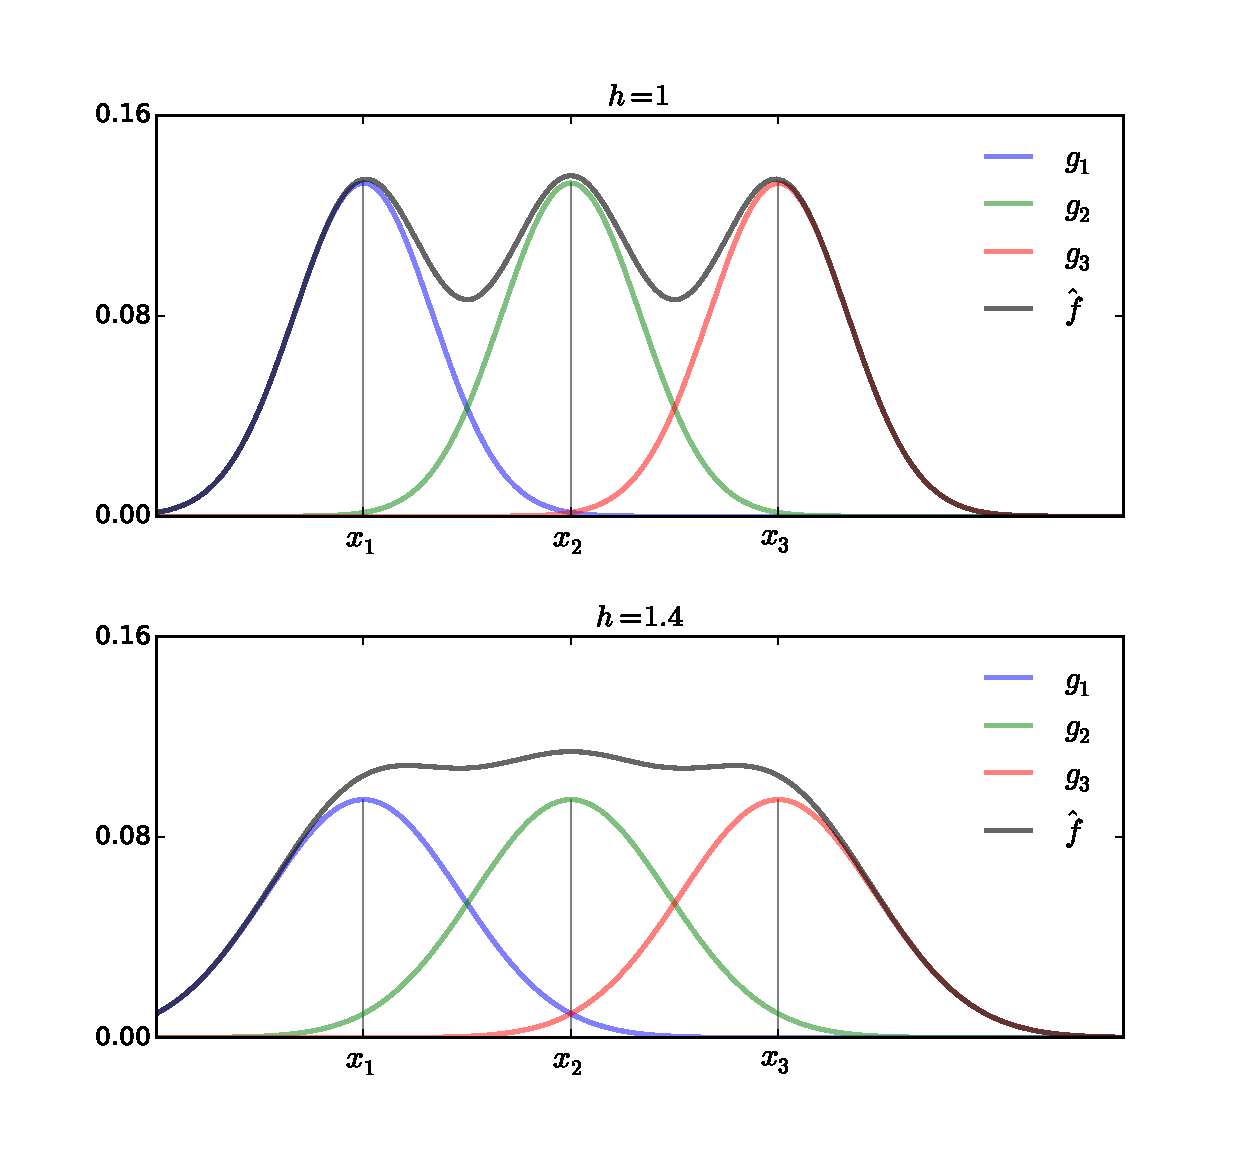
\includegraphics[trim={2em 2em 2em 2em}, clip]{npkde.pdf}}
    \caption{\label{f:npkde} Nonparametric KDE, different bandwidths}
    \end{figure}
    
\end{frame}

\begin{frame}

    \vspace{2em}
    Bandwidth adds smoothing to empirical distribution
    
    However, trade-off associated with
    smoothing
    \begin{itemize}
        \item as the bandwidth goes to zero,  kernel density becomes similar to the
        empirical distribution --- overfitting
        \item at the same time, excessive smoothing 
        adds too much bias, hiding  features of the true
        distribution
    \end{itemize}

    \vspace{.7em}
    Optimal bandwidth in terms of minimizing $L_p$ deviation depends on the unknown density $f$.
    
    Two  approaches: 
    \begin{itemize}
        \item  make assumptions on $f$ and choose the bandwidth
                accordingly
        \item cross-validation (we review below)
    \end{itemize}

\end{frame}

\begin{frame}

    \begin{figure}
    \centering
    \scalebox{.33}{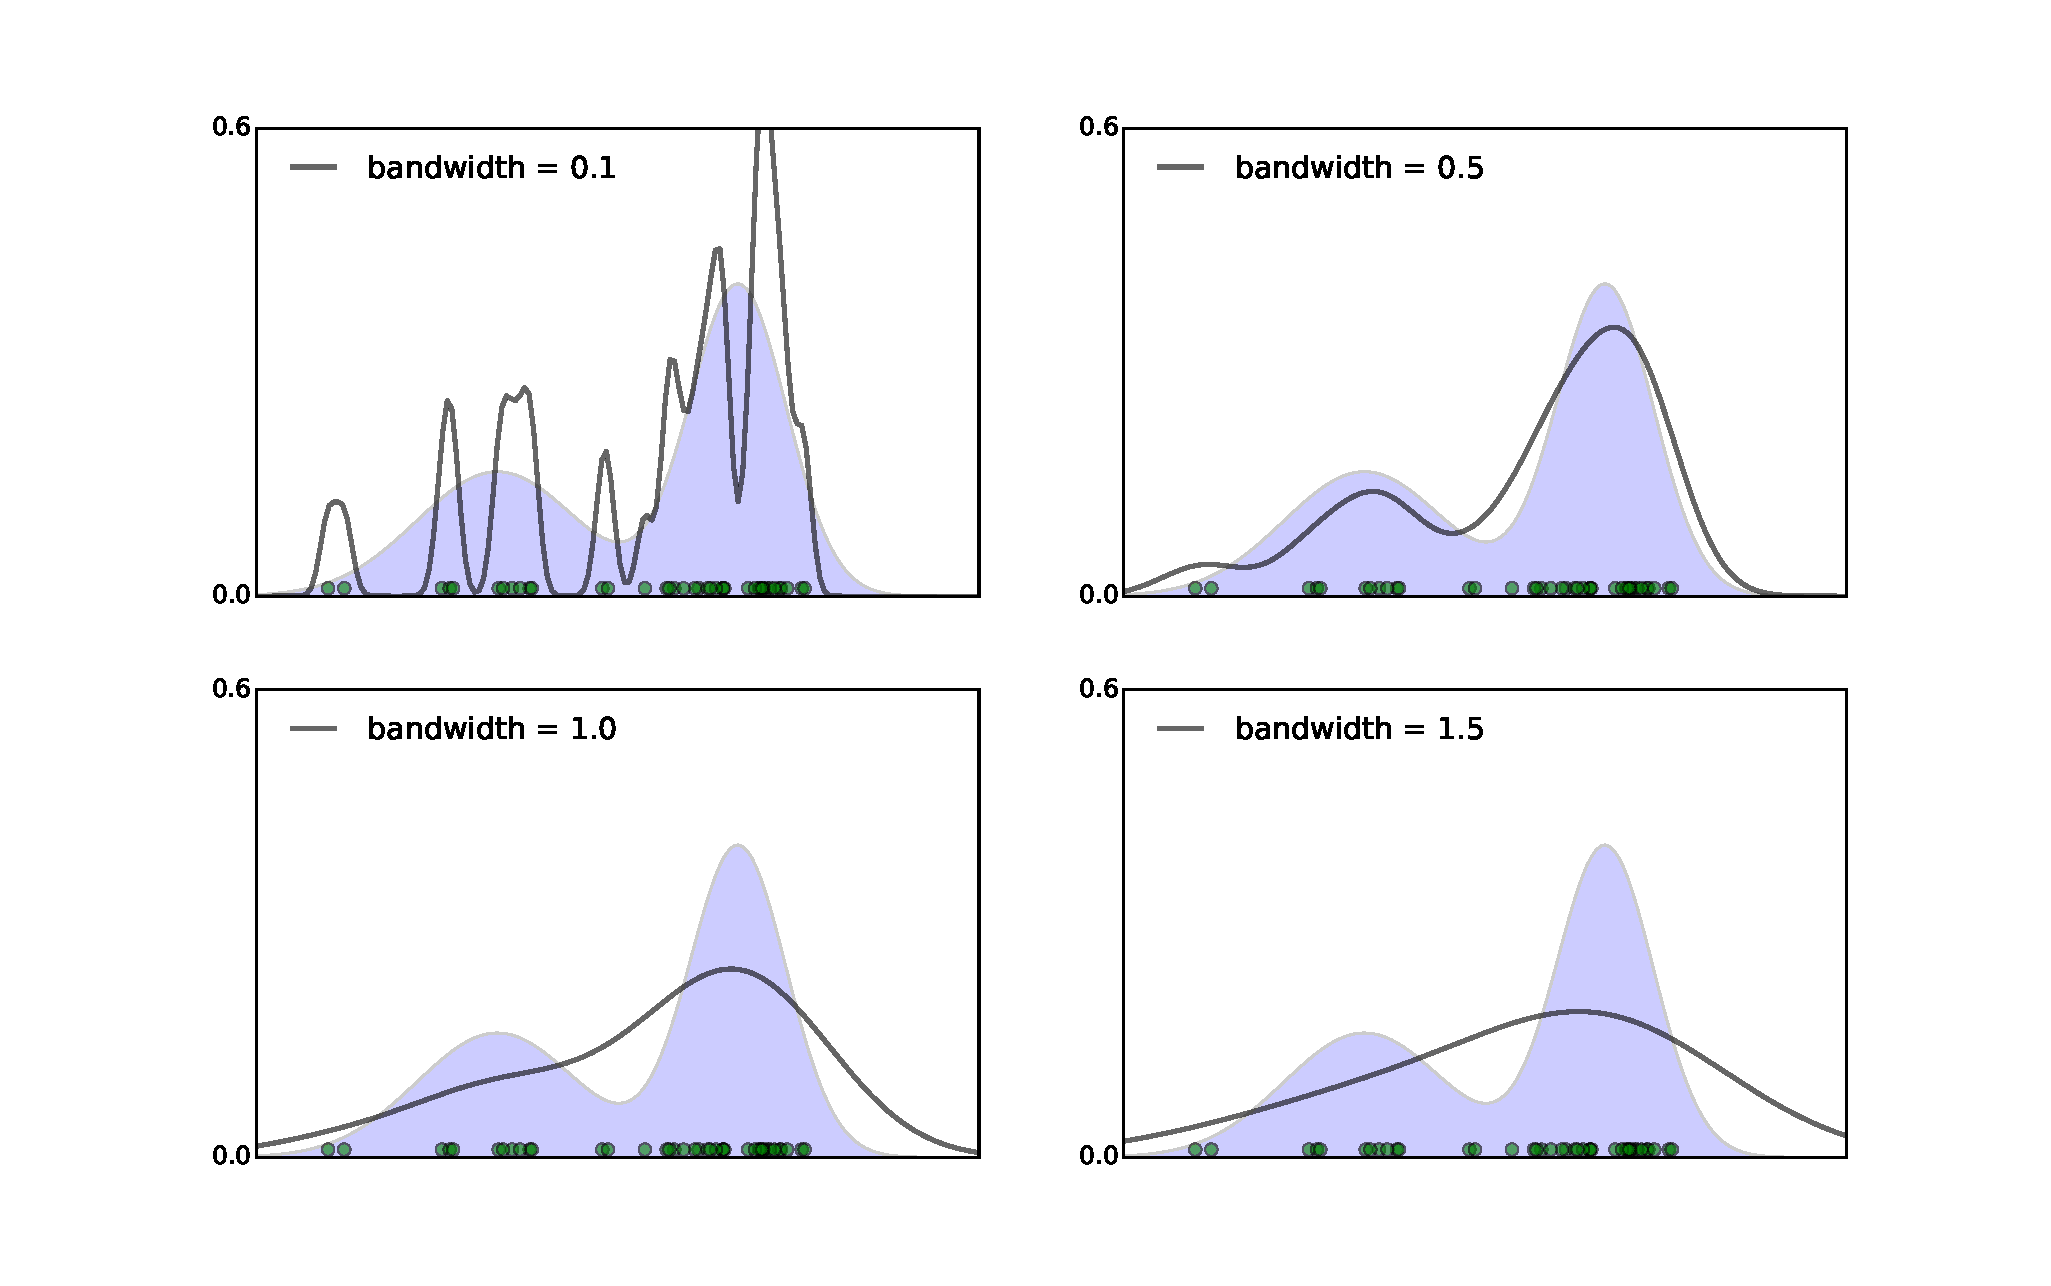
\includegraphics[trim={4em 4em 4em 4em}, clip]{one_dim_kde.pdf}}
    \caption{\label{f:one_dim_kde} Effect of changing the bandwidth}
    \end{figure}
    
\end{frame}

\begin{frame}{Theory of Kernal Density Estimation}

    \vspace{2em}
    Convolution of an
    arbitrary distribution $Q$ and a density $K$ on $\RR^d$ is the density on
    $\RR^d$ defined by
    %
    \begin{equation}
        \label{eq:gconv}
        (K \star Q) (\bolds') = \int K(\bolds' - \bolds) Q(\diff \bolds)
        \qquad (\bolds' \in \RR^d)
    \end{equation}
    
    \vspace{.7em}
    \Fact
    \eqref{ET-fa:ioc}
    For any density $K$ and arbitrary distribution $Q$ on $\RR^d$,
    the density $K \star Q$ equals $\lL(\boldx + \boldy)$ when 
        $\boldx$ and $\boldy $ are independent with $\lL(\boldx) = K$
        and $\lL(\boldy) = Q$
        
\end{frame}

\begin{frame}

    \vspace{2em}
    \Eg
    If $K = \nN(0, \sigma^2)$ for some $\sigma > 0$ and $Q$ is a
    distribution on $\RR$ that puts mass $q_n$ on points $s_1, \ldots,
    s_N$, then by \eqref{eq:gconv} 
    and the rule for integrating over discrete distributions 
    %
    \begin{equation}
        \label{eq:gconvd}
        (K \star Q)(s') = \sum_{n=1}^N K(s' - s_n) q_n
    \end{equation}
    
    
    This distribution is a mixture of normals

\end{frame}

\begin{frame}

    \vspace{2em}
    We are interested in convolutions induced
    by densities of the form
    %
    \begin{equation}
        \label{eq:kh}
        K_h(\bolds) := \frac{1}{h^d} K \left( \frac{\bolds}{h} \right)
    \end{equation}
    %
    where $K$ is any density and $h > 0$ is a parameter
    
    \vspace{.7em}
    The density
    $K_h$ in \eqref{eq:kh} is the density of
    $h \boldx$ when $\boldx$ is a random vector 
    on $\RR^d$ with density $K$
    
    \vspace{.7em}
    \Eg
    Figure on next slide shows the convolution of a tent-shaped
    distribution $Q$ and $K_h$ when $K$ is the standard normal density
    and $h$ takes different values

\end{frame}

\begin{frame}

    \begin{figure}
        \centering
        \scalebox{.44}{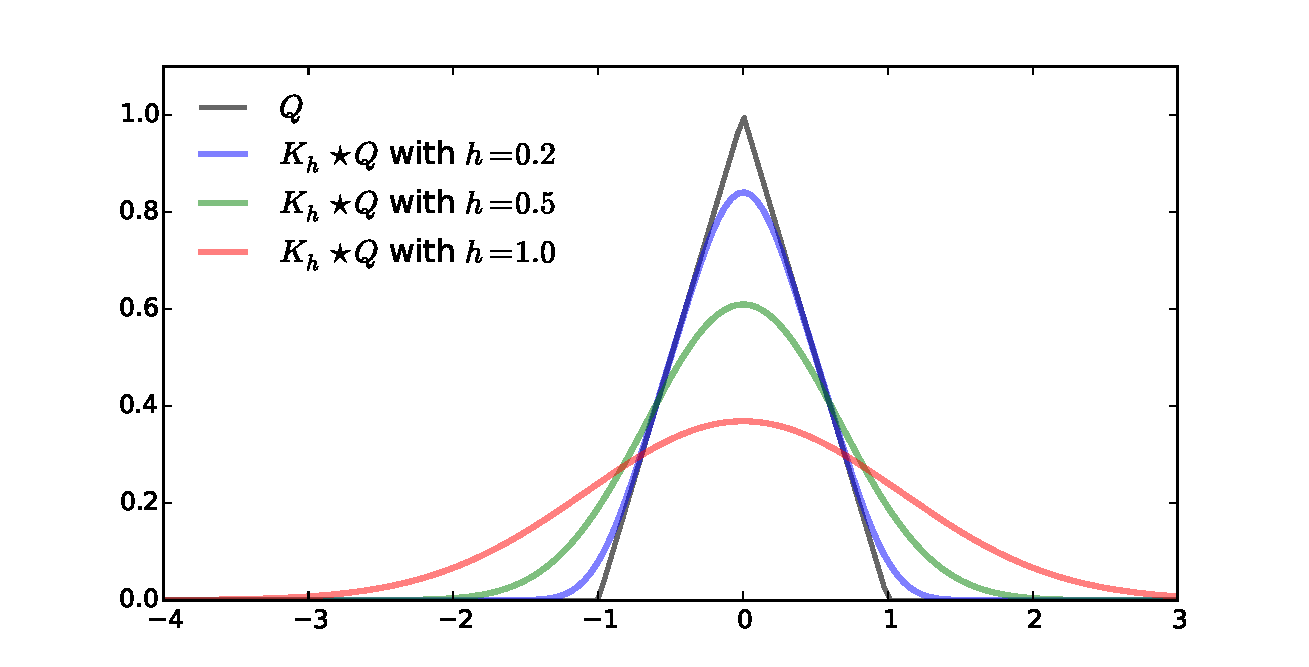
\includegraphics[trim={1em 0em 0em 1em}, clip]{convolve.pdf}}
        \caption{\label{f:convolve} Smoothing induced by convolutions}
    \end{figure}

\end{frame}

\begin{frame}

    \vspace{2em}
    \Fact
    \eqref{ET-fa:stz}
    Let $f$ and $K$ be any densities on $\RR^d$, and let $K_h$ be defined from
    $K$ via \eqref{eq:kh}.  If $f \in L_p$, then $K_h \star f \in L_p$, and 
    %
    \begin{equation*}
        \lim_{h \downarrow 0} \, \| K_h \star f - f \|_p = 0
    \end{equation*}
    %

\end{frame}

\begin{frame}\frametitle{Convolution and KDEs}

    \vspace{2em}
    Let $h$ be a positive number and let $K_h$ be as defined in \eqref{eq:kh}
    
    Rewrite the KDE in \eqref{eq:npkde}
        as $\hat f_N(\bolds) 
        = \frac{1}{N} \sum_{n=1}^N K_h(\bolds - \boldx_n)$
        
    $\hat P_N$ denotes the empirical distribution of the sample
    
    \vspace{.7em}
    Recalling expression for integrals with respect to $\hat P_N$, we can write 
    
    $$\hat f_N(\bolds') =  \int K_h(\bolds' - \bolds) \hat P_N(\diff \bolds)$$
    
    or, more simply, 
    %
    \begin{equation}
        \label{eq:kdeac}
        \hat f_N = K_h \star \hat P_N
    \end{equation}
    
    Adds smoothing to estimation of density using the sample analogue principle

\end{frame}

\begin{frame}

    \vspace{2em}
    For \emph{any} density $f$ and kernel $K$, the
    nonparametric kernel density estimator $\hat f_N$  is $L_1$-consistent for
    $f$
    
    Here we'll state and
    prove the corresponding $L_2$ result: 
    
    \vspace{.7em}
    \Thm
    \eqref{ET-t:kdec}
    Let $f$ and $K$ be densities on $\RR^d$ and elements of $L_2$.
    If
    %
    \begin{enumerate}
        \item $\{\boldx_n\}_{n \geq 1}$ is an {\sc iid} sequence of draws from
            $f$, and
        \item the bandwidth sequence $\{h_N\}$ satisfies $h_N \to 0$ and $N h_N^d \to \infty$ as $N \to \infty$,
    \end{enumerate}
    %
    then the sequence of density estimates $\{\hat f_N\}$ defined in \eqref{eq:npkde}
    is $L_2$-consistent for $f$.
    
\end{frame}

\begin{frame}
    
    \vspace{2em}
    For the remainder of this
    section, $\| \cdot \|$ is the $L_2$ norm and $h := h_N$
    
    Using the expression
    for $\hat f_N$ in \eqref{eq:kdeac} and the triangle inequality in
    \eqref{eq:lptri}, we have
    %
    \begin{equation}
        \label{eq:dnpk}
        \| \hat f_N - f \|
        \leq \| K_h \star \hat P_N - K_h \star f \| + \| K_h \star f - f \|
    \end{equation}

    \vspace{.7em}
    The first term is called the \navy{estimation error}
    \begin{itemize}
        \item  we only observe the empirical distribution
        $\hat P_N$ rather than the true distribution $f$
    \end{itemize}
    
    The second term called the \navy{approximation error} or \navy{bias}
    \begin{itemize}
        \item  caused
        by the smoothing we deliberately added to control the estimation error
    \end{itemize}
    
\end{frame}

\begin{frame}

    \vspace{2em}
    Condition 2. of theorem~\ref{ET-t:kdec}
    \begin{itemize}
        \item  $h_N \to 0$ shrinks the amount of smoothing as sample size 
                increases --- reducing approximation error as sample size increases
        \item $Nh_N^d \to \infty$ ensures smoothing not reduced too quickly, 
                controls estimation error

    \end{itemize}
    
    \Prf [Proof of theorem~\ref{ET-t:kdec}]
    
    By fact~\ref{ET-fa:stz}, the approximation error converges to zero
    under the conditions of theorem~\ref{ET-t:kdec}
    
    We now show the estimation error converges in probability to zero
    
\end{frame}

\begin{frame}

    \vspace{2em}
    \Prf (cont.)
    Fix $\delta >
    0$; by Chebyshev's inequality, we have
    %
    \begin{multline*}
        \PP \left\{ 
            \| K_h \star \hat P_N - K_h \star f \| \geq \delta 
            \right\} 
        \\ = \PP \left\{ 
            \| K_h \star \hat P_N - K_h \star f \|^2 \geq \delta^2 
              \right\} 
        \leq \frac{\xi_N}{\delta^2}
    \end{multline*}
    %
    where
    %
    \begin{equation*}
        \xi_N := 
            \EE \left\{
                \| K_h \star \hat P_N - K_h \star f \|^2
            \right\}
    \end{equation*}
    
    \vspace{.7em}
    To complete the proof,  we need show $\xi_N$
    converges to zero. Let 
    %
    \begin{multline*}
        \bar K_N (\bolds)
         := (K_h \star \hat P_N)(\bolds) - (K_h \star f)(\bolds) 
         \\ = \frac{1}{N} \sum_{n=1}^N
             \left\{
             K_h(\bolds - \boldx_n) - \EE [ K_h(\bolds - \boldx_n) ]
             \right\}
    \end{multline*}
    
    \end{frame}
    %
    \begin{frame}
    \Prf (cont.)
    We can then write
    %
    \begin{equation}
        \label{eq:hktz}
        \xi_N
        =
        \EE \left\{ 
            \int \left[ \bar K_N(\bolds) \right]^2 
            \diff \bolds
            \right\}
        =
        \int 
        \EE \left\{ \left[ \bar K_N(\bolds) \right]^2 \right\}
            \diff \bolds
    \end{equation}
    
    \vspace{.7em}
    (The interchange of order of expectation and integration
    is valid for nonnegative integrands)
    
    \vspace{.7em}
    Since $\bar K_N (\bolds)$ is the sample mean of $N$
    {\sc iid} zero-mean random variables, we have
    %
    \begin{equation*}
        \EE \left\{ \left[ \bar K_N(\bolds) \right]^2 \right\}
        = \var  \left[ \bar K_N(\bolds) \right]
        = \frac{1}{N} \var[ K_h(\bolds - \boldx_n) ]
    \end{equation*}
    %

\end{frame}


\begin{frame}

    \vspace{2em}
    \Prf (cont.)
    Moreover 
    %
    \begin{multline*}
    \var[ K_h(\bolds - \boldx_n) ]
    = \EE \left\{ [ K_h(\bolds - \boldx_n) ]^2 \right\}
    - \left\{ \EE[ K_h(\bolds - \boldx_n)]  \right\}^2
    \\ \leq 
    \EE \left\{ [ K_h(\bolds - \boldx_n) ]^2 \right\}
    \end{multline*}
    %
    In summary,
    %
    \begin{equation*}
        \label{eq:xintz}
        \xi_N \leq 
        \frac{1}{N}
        \int 
        \EE \left\{ [ K_h(\bolds - \boldx_n) ]^2 \right\}
            \diff \bolds
    \end{equation*}
    
    \vspace{.7em}
    Switching the order of integration,
    %
    \begin{equation*}
        \int 
        \EE \left\{ [ K_h(\bolds - \boldx_n) ]^2 \right\}
            \diff \bolds
        =
        \int 
        \left\{
            \int [ K_h(\bolds - \bolds') ]^2 \diff \bolds
        \right\}
            f(\bolds') \diff \bolds'
    \end{equation*}
    %

\end{frame}

\begin{frame}

    \vspace{2em}
    \Prf (cont.)
    From the definition of $K_h$ and a change of variable argument,
    %
    \begin{equation*}
        \int [ K_h(\bolds - \bolds') ]^2 \diff \bolds
         = \frac{1}{h^{2d}}
            \int \left[ K \left( 
            \frac{\bolds - \bolds'}{h} 
                     \right) 
                 \right]^2 \diff \bolds
         = \frac{1}{h^d}
            \int [ K (\boldu) ]^2 \diff \boldu
    \end{equation*}
    %
    Putting this together with \eqref{eq:xintz} gives the bound
    %
    \begin{equation*}
        \xi_N 
        \leq 
        \int 
        \frac{1}{Nh^d} \, \| K \|^2  \, f(\bolds') \diff \bolds'
        = \frac{1}{Nh^d}  \,\| K \|^2 
    \end{equation*}
    %
    The term $\| K \|^2 := \| K \|^2_2$ is finite by assumption
    
    Recalling $Nh^d =
    Nh^d_N \to \infty$, we see $\xi_N \to 0$ as required \qedsymbol
    
\end{frame}

\begin{frame}

    \vspace{2em}
    Parametric techniques excel when we have knowledge about parametric
    classes and specific functional forms --- from underlying theory 
    \begin{itemize}
        \item this is more difficult in economics and other social sciences 
        --- makes non-parametric techniques more attractive 
    \end{itemize}

    \vspace{.7em}
    Nonparametric methods do not solve all our problems
    \begin{itemize}
        \item theoretical results presented above are purely asymptotic
        \item strong finite sample
        results require strict assumptions on the target density
        \item no uniform rate of convergence for all target densities
    \end{itemize}
    
\end{frame}

\begin{frame}

    \vspace{2em}
    Nonparametric
    methods have relatively little structure in the form of prior knowledge and hence
    require abundant data

\end{frame}

\section{Controlling Complexity}

\begin{frame}\frametitle{Ridge Regresion}
    
    \vspace{2em}
    Turn attention to finite sample
    properties
    
    Ridge regression --- a popular
    method of estimation in both econometrics and machine learning 
    
    \vspace{.7em}
    Ridge regression connects to ideas at
    the heart of finite sample theory
    \begin{itemize}
        \item complexity
        \item prior knowledge
        \item  bias--variance trade-off
    \end{itemize}
    
\end{frame}

\begin{frame}

    \vspace{2em}
    Start with the OLS setting with assumptions~\ref{ET-a:lols}--\ref{ET-a:bols2}
    
    Recall the usual OLS estimator $\hboldbeta$ 
    %
    \begin{equation*}
        \hboldbeta = \argmin_{\boldb \in \RR^K} \sum_{n=1}^N (y_n - \boldx_n^\T \boldb)^2
    \end{equation*}
    
    \vspace{.7em}
    OLS estimator minimizes the
    empirical risk under quadratic loss when the hypothesis space is
    the set of linear functions
    
    Under our assumptions, the OLS estimator: 
    \begin{itemize}
        \item unbiased for $\boldbeta$
        \item has the lowest variance among all linear unbiased estimators of
    $\boldbeta$
    \end{itemize}
    
\end{frame}

\begin{frame}

    \vspace{2em}
    More natural way
    to evaluate estimators is to consider their mean squared error
    
    Define the MSE of an estimator $\hat \boldb$ of $\boldbeta$ as
    %
    \begin{equation*}
        \mse(\hat \boldb, \boldbeta) := \EE \left\{ \| \hat \boldb - \boldbeta \|^2  \right\}
    \end{equation*}
    
    Alternatively,
    %
    \begin{equation}
        \label{eq:dmse2}
        \mse(\hat \boldb, \boldbeta) 
        = \EE \left\{ \|  \, \hat \boldb - \EE[\hat \boldb] \, \|^2 \right\}
            + \| \, \EE[\hat \boldb] - \boldbeta \, \|^2 
    \end{equation}
    
    \vspace{.7em}
    Minimization of MSE involves a trade-off between
    \begin{enumerate}
        \item variance term
        \item bias term 
    \end{enumerate}
    
\end{frame}

\begin{frame}

    \vspace{2em}
    There
    exists a biased linear estimator with lower mean squared error than
    $\hboldbeta$
    
    The estimator is the solution to the modified least
    squares problem 
    %
    \begin{equation}
        \label{eq:rrp}
        \min_{\boldb \in \RR_K}
        \left\{
         \sum_{n=1}^N (y_n - \boldx_n^\T \boldb)^2 + \lambda \| \boldb \|^2
         \right\}
    \end{equation}
    %
    where $\lambda \geq 0$ is called the \navy{regularization parameter}
    
    \vspace{.7em}
    Minimizing the empirical risk plus a term that
    penalizes large values of $\| \boldb \|$
    
    The solution to \eqref{eq:rrp} is
    %
    \begin{equation}
        \label{eq:rrs}
        \hboldbeta_{\lambda} 
            := (\boldX^\T \boldX + \lambda \boldI)^{-1} \boldX^\T \boldy
    \end{equation}
    
\end{frame}

\begin{frame}
    
    \vspace{2em}
    The estimator $\hboldbeta_{\lambda}$ is called the \navy{ridge regression
    estimator}. Note: 
    %
    \begin{enumerate}
        \item $\hboldbeta_\lambda$ is the OLS estimator when $\lambda = 0$ and
        \item $\hboldbeta_\lambda$ is biased whenever $\lambda > 0$ (ex.~\ref{ET-ex:rrbiased})
    \end{enumerate}
   
   \vspace{.7em}
       \Thm
        \eqref{ET-t:rrg}
        Under the OLS assumptions~\ref{ET-a:lols}--\ref{ET-a:bols2}, there exists a
        $\lambda > 0$ such that 
        %
        \begin{equation*}
            \mse \left(\hboldbeta_{\lambda}, \boldbeta \right) < 
            \mse \left( \hboldbeta, \boldbeta \right)
        \end{equation*}
        %
    Proof is in \cite{hoerl1970ridge}

\end{frame}

\begin{frame}

    \vspace{2em}
    Traditional view of ridge regression:
    \begin{itemize}
        \item OLS assumptions valid, however,
    instances where $\boldX^\T \boldX$ is almost singular due to strong
    correlation between regressors
    \item in this case, inverting
    $\boldX^\T \boldX$ is numerically unstable
    \item stabilize the inversion by
        adding some positive value of $\lambda$
    \end{itemize}
    
\end{frame}

\begin{frame}
    
    \vspace{2em}
    Here's another view of ridge regression:
    \begin{itemize}
        \item standard OLS assumptions are implausible
        \item obtaining the regression function $f^*$ (an infinite dimensional object)
        with a finite amount of data is ill-posed
        \item regularization term in ridge regression manages complexity of the
            candidate functions used to approximate the regression function
    \end{itemize}
    

\end{frame}
    

\begin{frame}\frametitle{Tikhonov Regularization}

    \vspace{2em}
    Least squares estimator  the solution to an overdetermined
    system of equations
    
    Solving ill-posed
    linear systems in high dimensions: \emph{any attempt to back
    out or infer a complex object by solving a system about which we have limited
    information requires a degree of regularization}
    
    \vspace{.7em}
    To illustrate, suppose 
    %
    \begin{enumerate}
        \item $\boldA \boldb = \boldc$ is an overdetermined system, where $\boldA$
            is $N \times K$ with $N > K$
        \item due to measurement error, we only observe an approximation
            $\boldc_0$ of $\boldc$
        \item $\boldb^*$ is the (unobservable) least squares solution $\argmin_{\boldb} \| \boldA \boldb - \boldc \|^2$
    \end{enumerate}

\end{frame}

\begin{frame}

    \vspace{2em}
    Natural approach to approximating
    $\boldb^*$ is to solve $\boldA \boldb = \boldc_0$ by least squares
    
    Another approach to solve the above problem: 
    %
    \begin{equation*}
        \label{eq:mla}
       m(\lambda) := \| \boldA \boldb - \boldc_0 \|^2 + \lambda \| \boldb \|^2  
    \end{equation*}
    %
    for some small but positive $\lambda$
    
    \vspace{.7em}
    This approach called \navy{Tikhonov regularization}
    \begin{itemize}
        \item minimizing least squares plus a
    penalty term
    \end{itemize}
    
\end{frame}

\begin{frame}

    \vspace{2em}
    Simulation where $\boldA$ chosen stochastically but with a
    tendency towards multicollinearity
    \begin{itemize}
        \item first set $\boldb^* := (10,10,\ldots,10)^\T$
        \item then set $\boldc := \boldA
    \boldb^*$
    \end{itemize}
    
    \vspace{.7em}
    By construction, $\boldb^*$ is a solution to the system
    $\boldA \boldb^* = \boldc$, and also the least squares solution
    
    The figure on next slide shows 10 solutions each for the ordinary
    and regularized solutions,
    corresponding to 10 draws of $\boldc_0$
    
\end{frame}

\begin{frame}

    \begin{figure}
       \begin{center}
        \scalebox{.44}{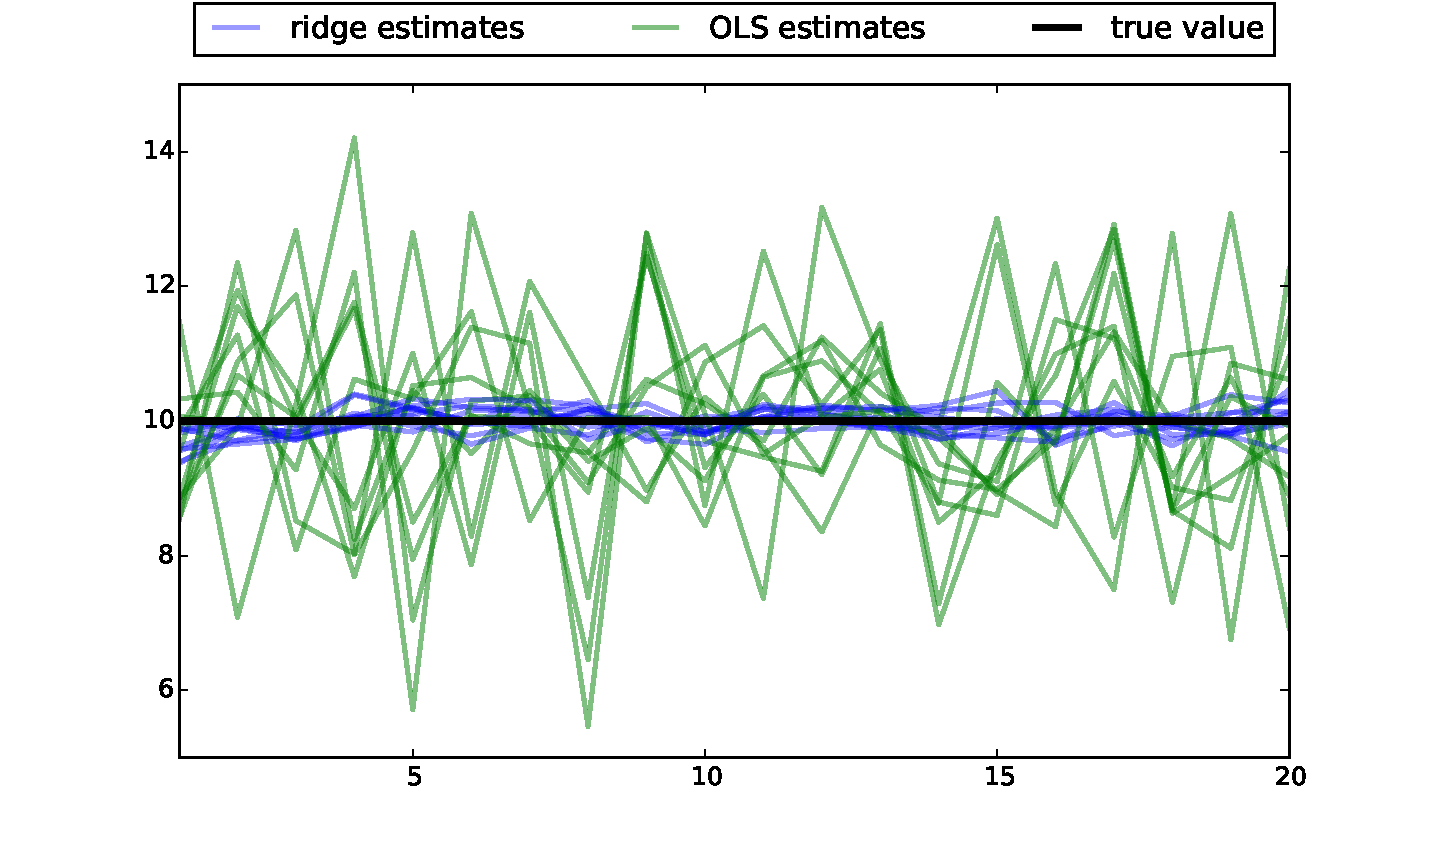
\includegraphics{tikreg.pdf}}
        \caption{\label{f:tikreg} Effect of Tikhonov regularization, $\lambda=1$}
       \end{center}
    \end{figure}
    
\end{frame}


\begin{frame}\frametitle{Subset Selection and Ridge Regression}

    Problem of \navy{subset
    selection}
    \begin{itemize}
        \item  which variables to
    include in a regression? 
        \item choose the right set of basis functions
    \end{itemize}
    
    Subset selection a version of the empirical risk minimization problem


\end{frame}

\begin{frame}
    
    \vspace{2em}
    Suppose we have output $y$ and inputs
    $\boldx \in \RR^K$ --- $\boldx$ contains $K$ candidate
    regressors
    
    To include all regressors, minimize
    empirical risk over $\llL$, the hypothesis space of
    linear functions from $\RR^K$ to $\RR$
    
    \vspace{.7em}
    To exclude some subset of
    regressors, set $I \subset \{1,\ldots,K\}$ to be the set of indices of
    the regressors we want to exclude and regress $y$ on the remainder
    
    Equivalent to minimizing the empirical risk over the hypothesis space
    %
    \begin{equation*}
        \hH_{-I} := \left\{
            \text{ all functions } 
                f(\boldx) = \boldb^\T \boldx
                \text{ with }
                b_k = 0 \text{ for all } k \in I
               \right\}
    \end{equation*}
    
\end{frame}

\begin{frame}

    \vspace{2em}
    The subset selection problem has been tackled by many researchers
        \begin{itemize}
            \item Akaike Information Criterion (AIC)
            \item  Bayesian Information Criterion (BIC)
            \item  Mallow's $C_p$ statistic
        \end{itemize}
    
    \vspace{.7em}
    $K$ regressors means $2^K$
    subsets--- to avoid computational burden, use ridge regression:
    \begin{itemize}
        \item regularization term leads us to choose an estimate with smaller norm
        \item the coefficients of less helpful regressors are
    driven towards zero
        \item reduces model selection problem to tuning a single
    parameter
    \end{itemize}
    \
\end{frame}

\begin{frame}

    \vspace{2em}
    Reconsider the problem of mapping a single co-variate $x$ 
    into $\phi(x) = (1,x, x^{2},\dots, x^{d})$ and regressing 
    $y$ on $\phi(x)$
    
    The hypothesis
    spaces were the sets $\pP_d$ of degree $d$ polynomials for different values of
    $d$
    
    \vspace{.7em}
    For each $d$ we minimized the empirical risk over $\pP_d$, which
    translates into solving 
    %
    \begin{equation*}
        \min_{\boldb} \sum_{n=1}^N 
            \left[ y_n - \boldb^\T\boldphi(x_n) \right]^2
            \quad \text{where} \quad
            \boldphi(x) = (x^0, x^1,\ldots, x^d)
    \end{equation*}
    %
    Choosing the right $d$ isomorphic to subset selection
    
\end{frame}

\begin{frame}

    \begin{figure}
       \begin{center}
        \scalebox{.44}{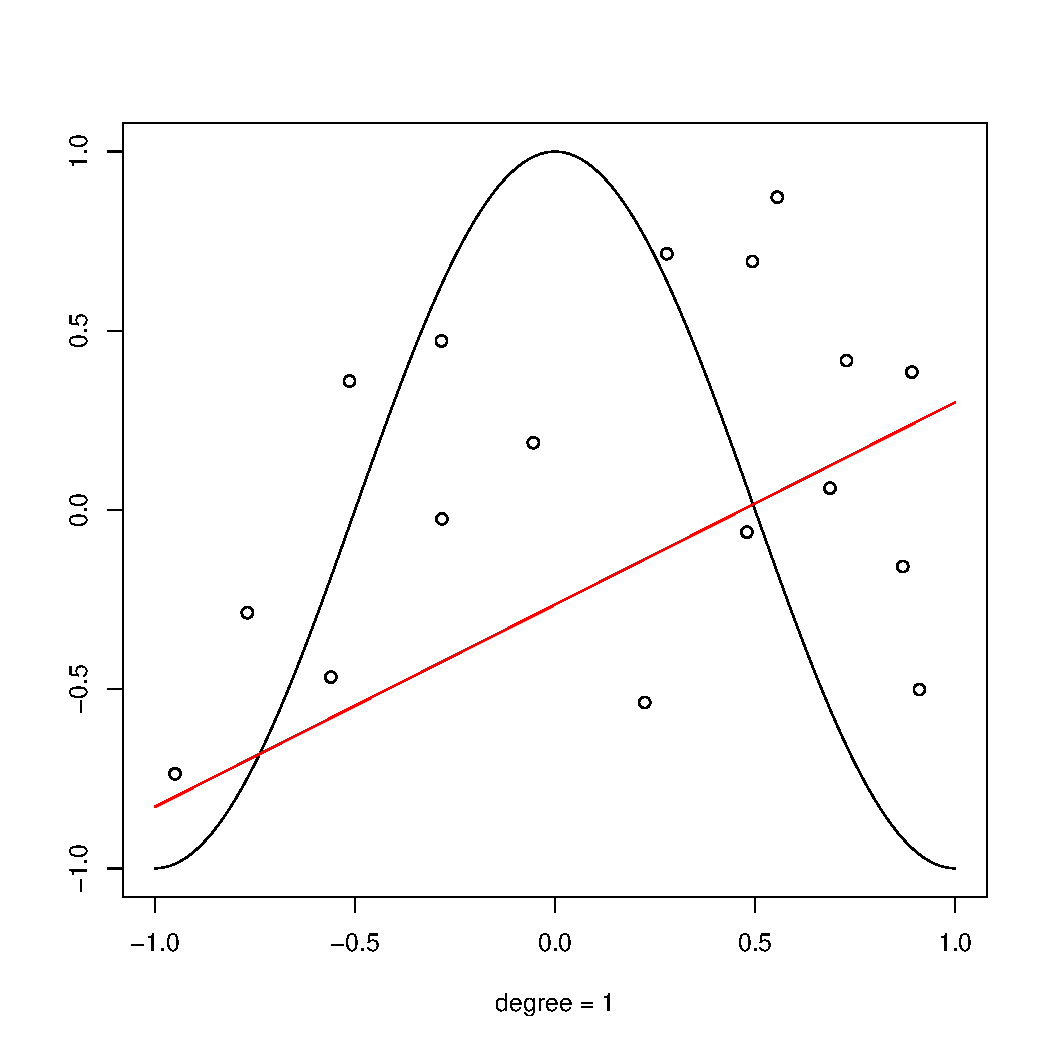
\includegraphics[trim={0em 0em 0em 2em}, clip]{ofit1.pdf}}
        \caption{\label{f:ofit1} Fitted polynomial, $d=1$}
       \end{center}
    \end{figure}
    
\end{frame}

\begin{frame}

    \begin{figure}
       \begin{center}
        \scalebox{.44}{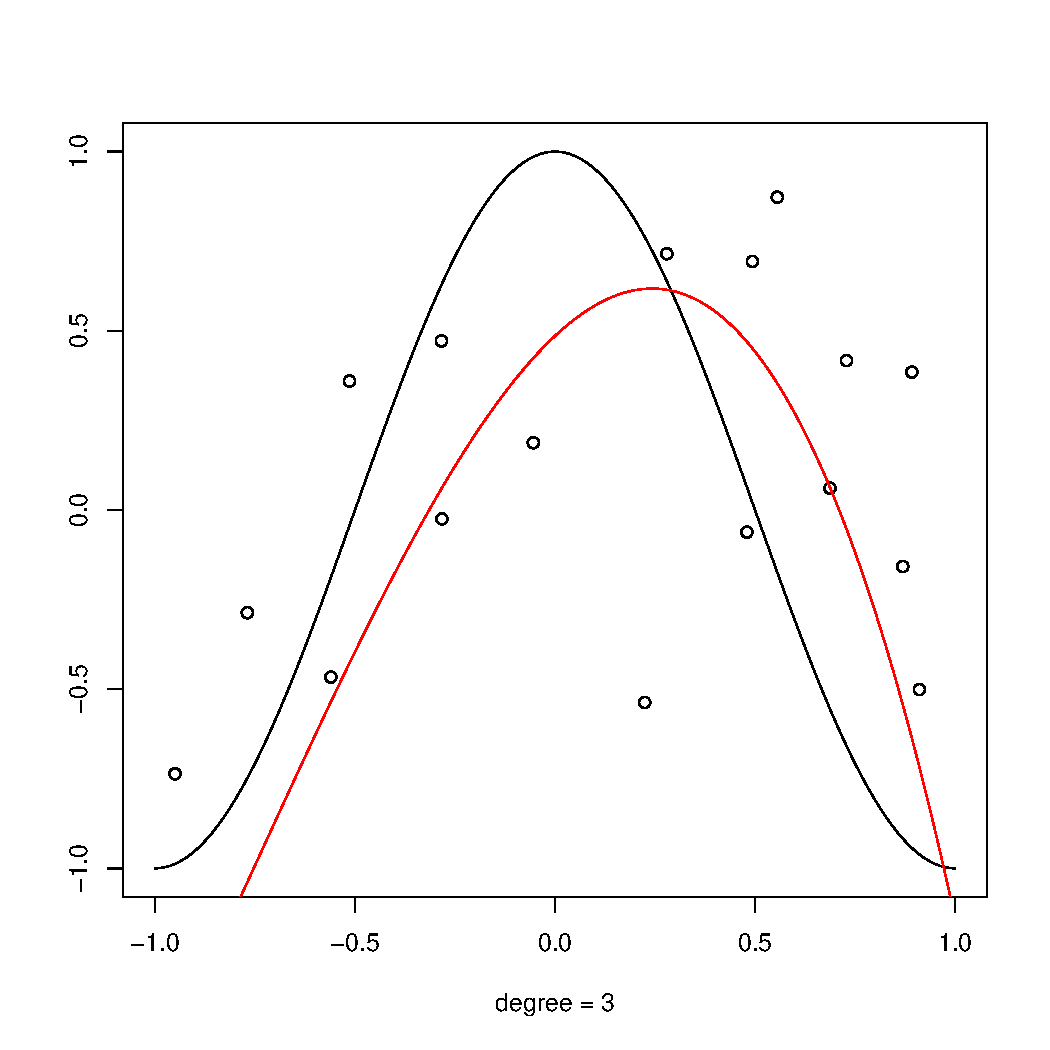
\includegraphics[trim={0em 0em 0em 2em}, clip]{ofit3.pdf}}
        \caption{\label{f:ofit3} Fitted polynomial, $d=3$}
       \end{center}
    \end{figure}
    
\end{frame}

\begin{frame}

    \begin{figure}
       \begin{center}
        \scalebox{.44}{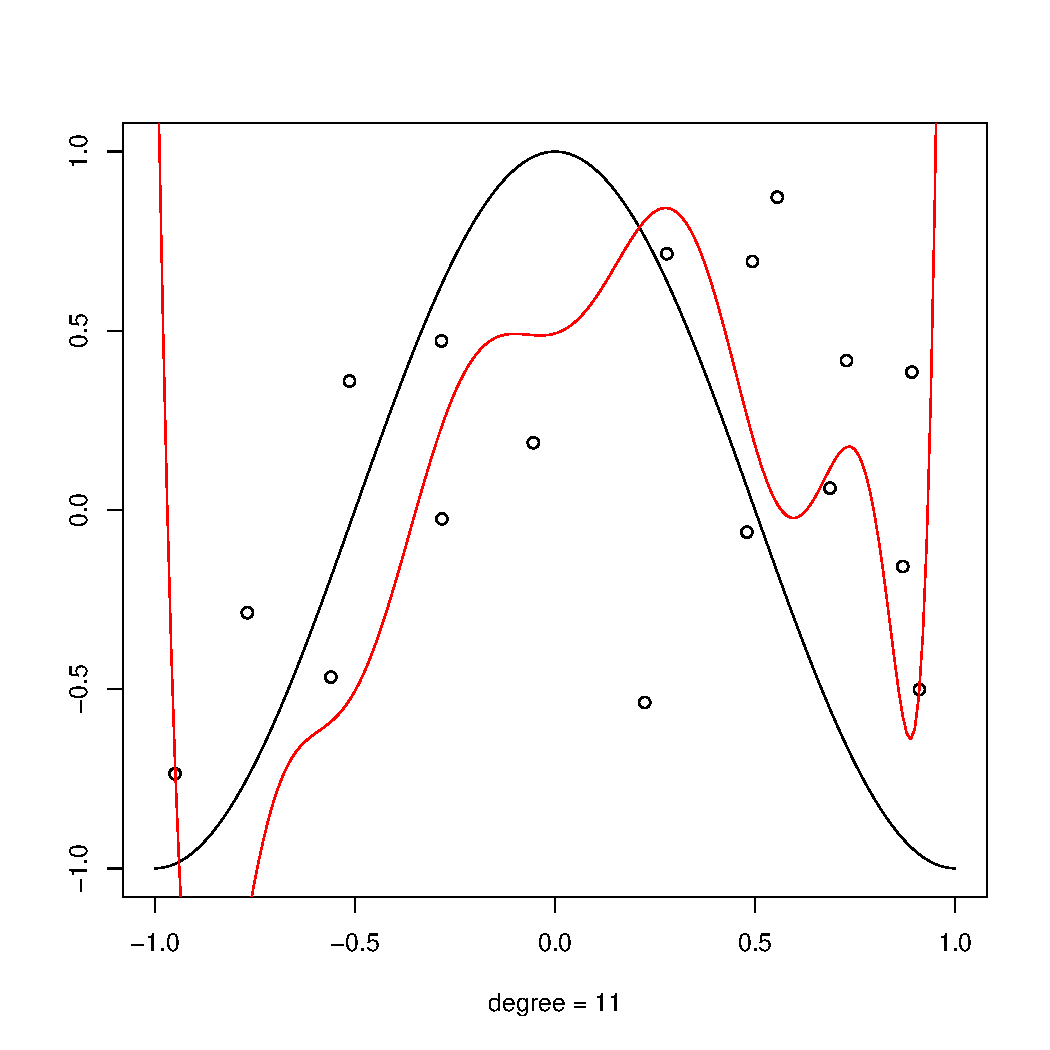
\includegraphics[trim={0em 0em 0em 2em}, clip]{ofit11.pdf}}
        \caption{\label{f:ofit11} Fitted polynomial, $d=11$}
       \end{center}
    \end{figure}
    
\end{frame}

\begin{frame}

    \begin{figure}
       \begin{center}
        \scalebox{.44}{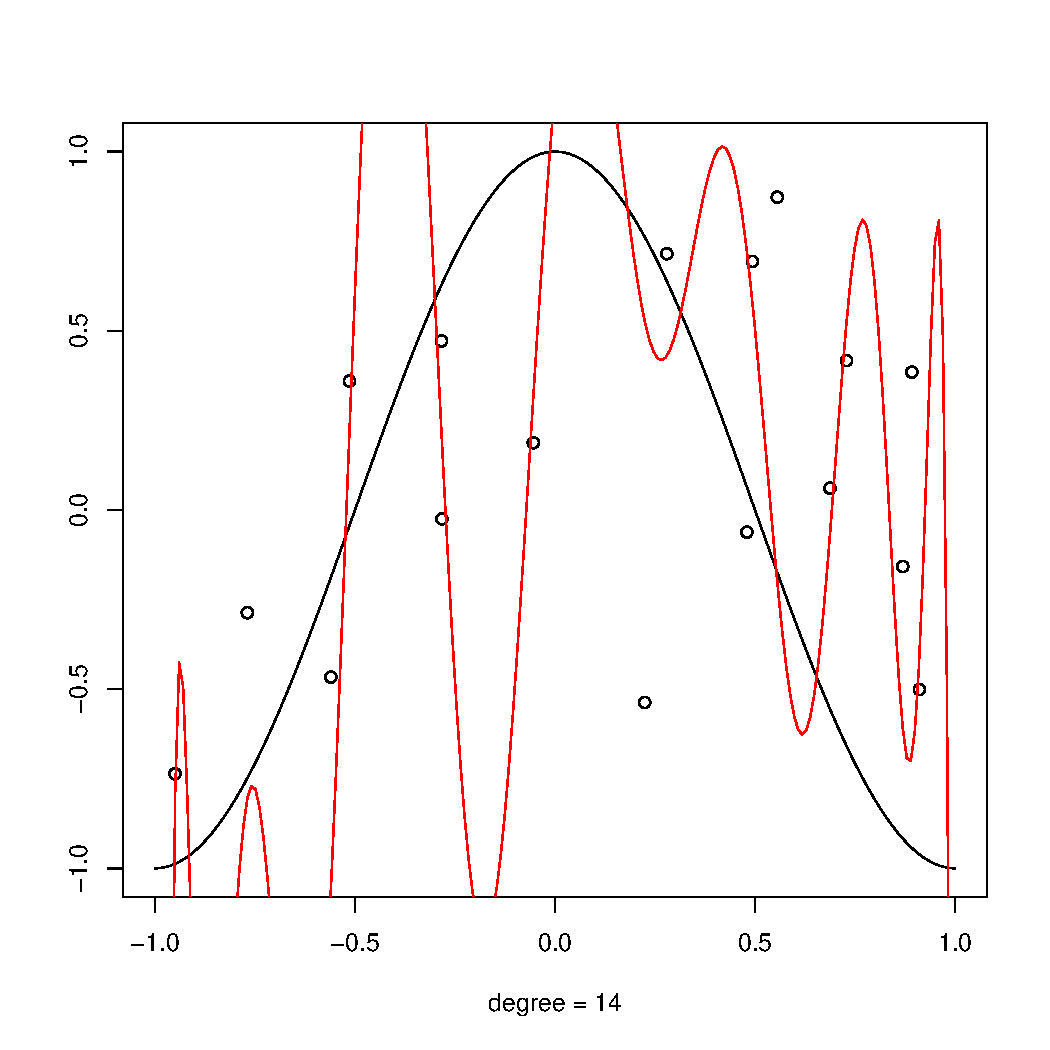
\includegraphics[trim={0em 0em 0em 2em}, clip]{ofit14.pdf}}
        \caption{\label{f:ofit14} Fitted polynomial, $d=14$}
       \end{center}
    \end{figure}
    
\end{frame}

\begin{frame}

    \vspace{2em}
    To use ridge regression for the problem
    
    First, take
    $\pP_{14}$ as our hypothesis space
    \begin{itemize}
        \item large enough to
    provide a good fit to the data, but we have overfitting 
    \end{itemize}
    
    \vspace{.7em}
    Solve the regularization problem
    %
    \begin{equation*}
        \min_{\boldb} \sum_{n=1}^N 
            \left\{
                \left[ y_n - \boldb^\T\boldphi(x_n) \right]^2 + \lambda \| \boldb \|^2
            \right\}
    \end{equation*}
    %
    for different values of $\lambda$

\end{frame}

\begin{frame}

    \begin{figure}
   \begin{center}
    \scalebox{.44}{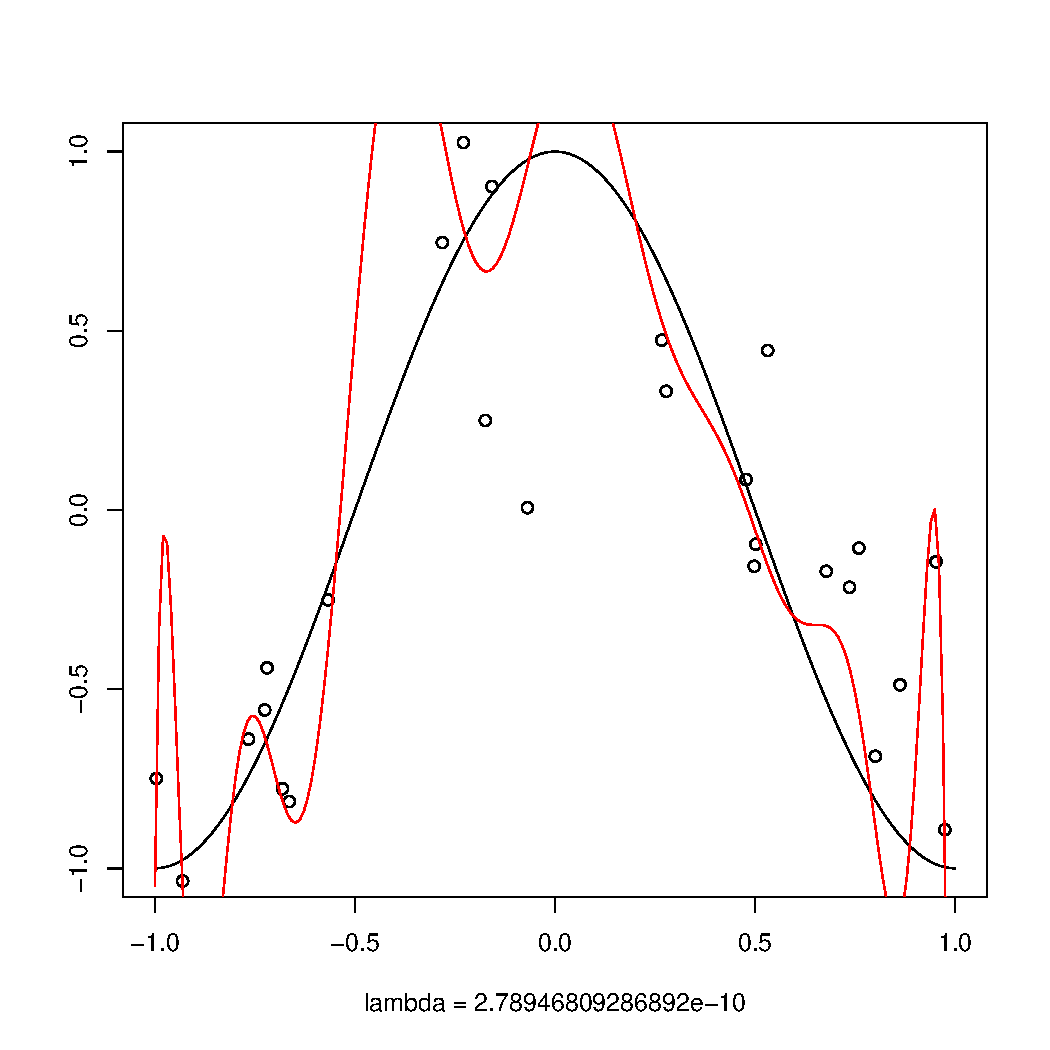
\includegraphics[trim={0em 1em 0em 3em}, clip]{ridge_plots/ridgeplot1.pdf}}
    \caption{\label{f:ridgeplot1} Fitted polynomial, $\lambda \approx 0$}
   \end{center}
    \end{figure}
    
\end{frame}

\begin{frame}

    \begin{figure}
   \begin{center}
    \scalebox{.44}{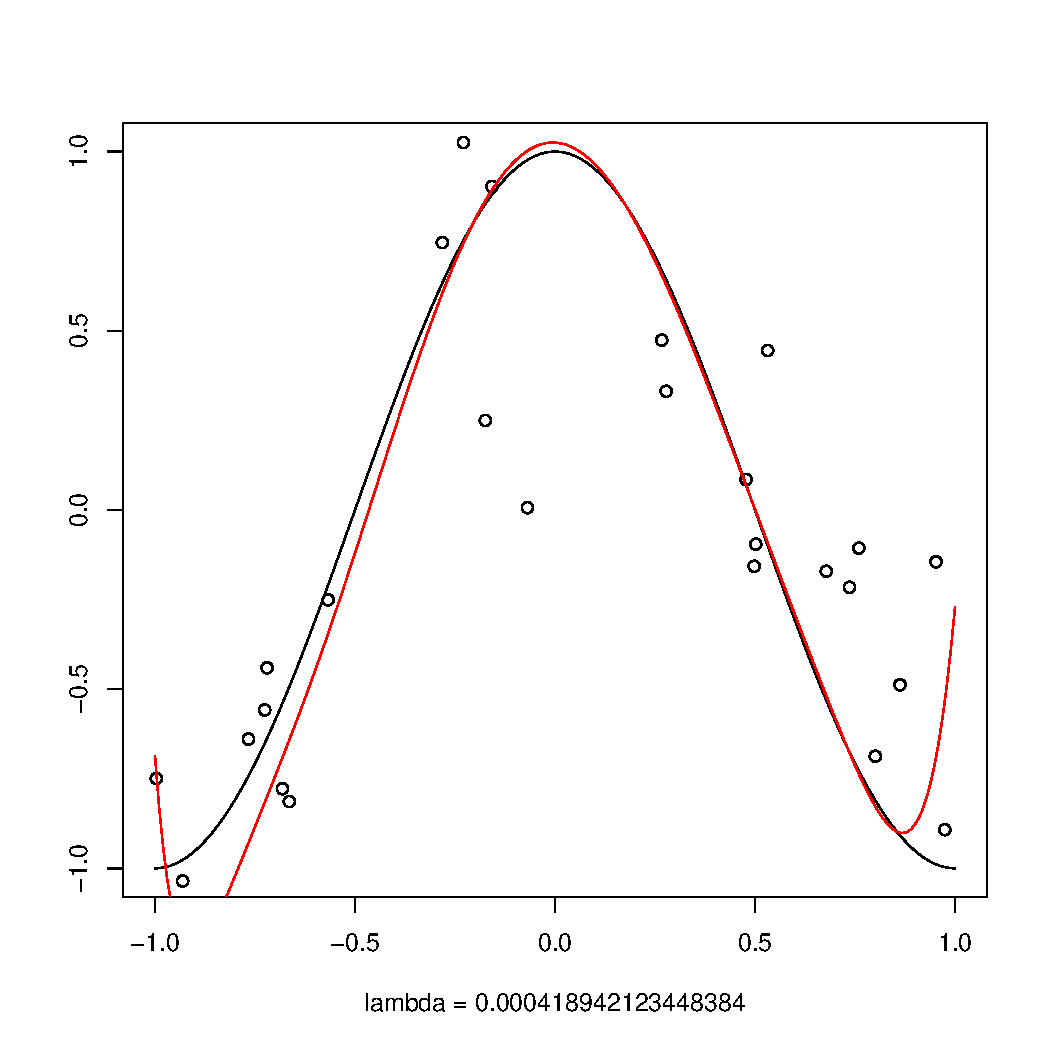
\includegraphics[trim={0em 1em 0em 3em}, clip]{ridge_plots/ridgeplot5.pdf}}
    \caption{\label{f:ridgeplot5} Fitted polynomial, $\lambda \approx 0.0004$}
   \end{center}
    \end{figure}

\end{frame}

\begin{frame}

    \begin{figure}
   \begin{center}
    \scalebox{.44}{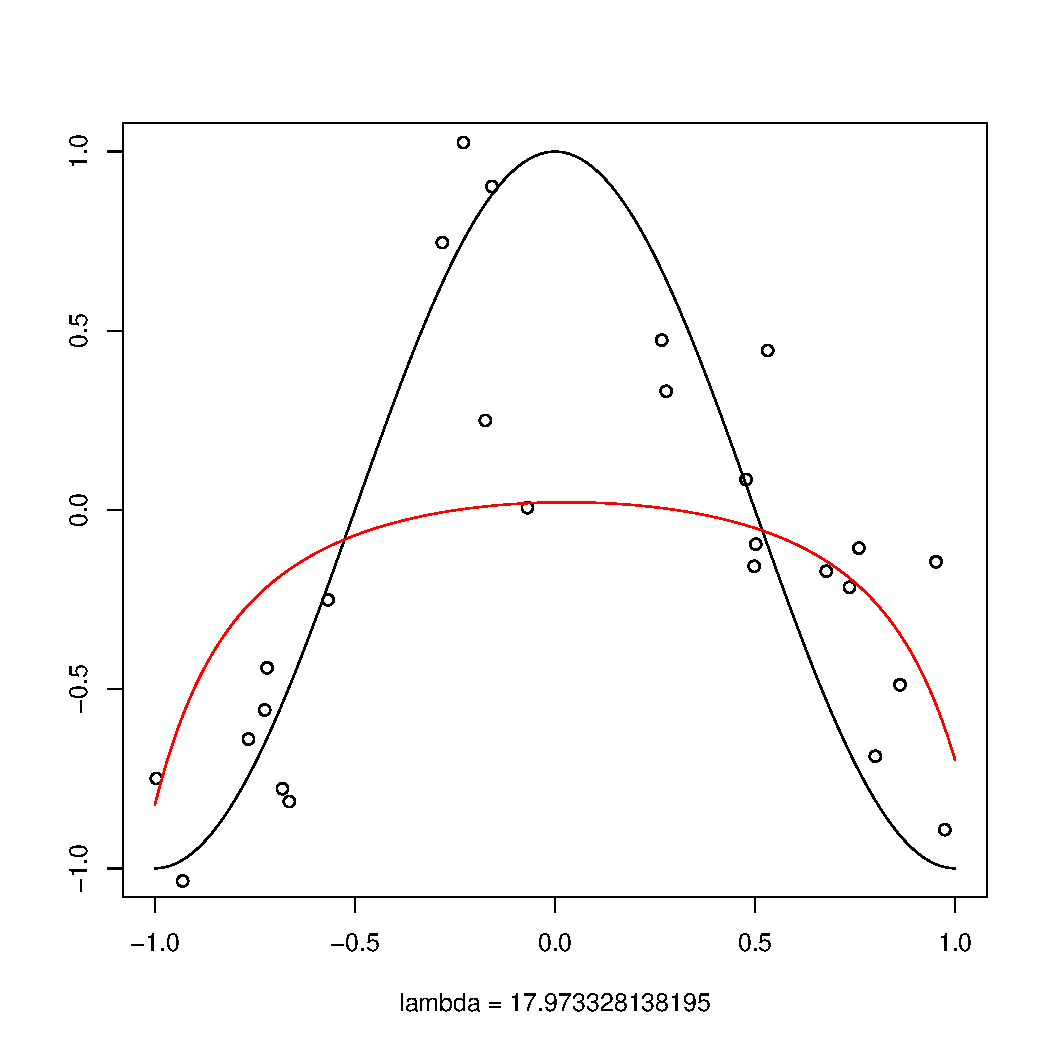
\includegraphics[trim={0em 1em 0em 3em}, clip]{ridge_plots/ridgeplot8.pdf}}
    \caption{\label{f:ridgeplot8} Fitted polynomial, $\lambda \approx 18$}
   \end{center}
    \end{figure}
    
\end{frame}

\begin{frame}

    \begin{figure}
   \begin{center}
    \scalebox{.42}{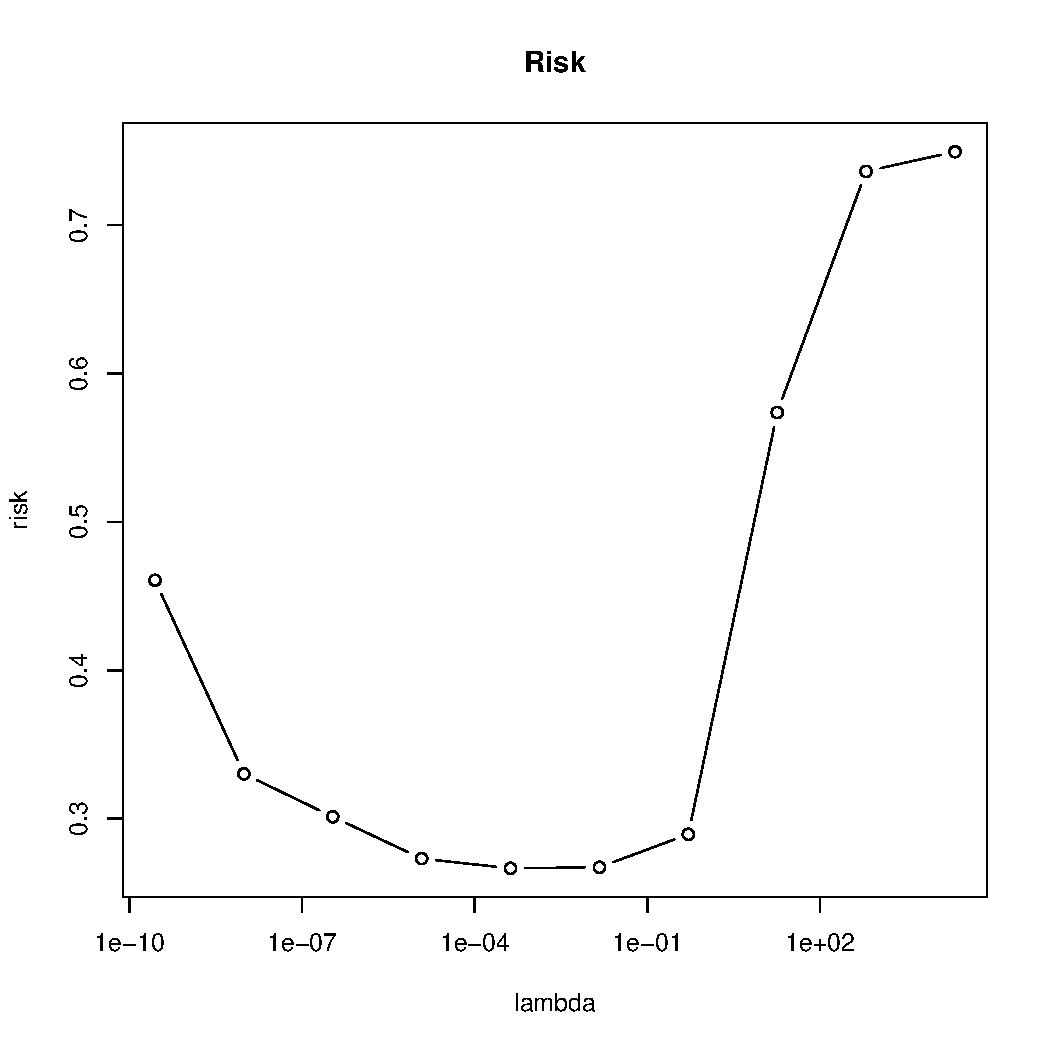
\includegraphics[trim={0em 1em 0em 2em}, clip]{ridge_risk.pdf}}
    \caption{\label{f:ridge_risk} Risk of $\hat f_{\lambda}$ plotted against $\lambda$}
   \end{center}
    \end{figure}
    
\end{frame}

\begin{frame}\frametitle{Bayesian Methods and Regularization}
    
    \vspace{2em}
    Bayesian analysis provides method for including prior information into statistical estimation
    
    \vspace{.7em}
    Prior information can be 
    \begin{itemize}
        \item guidance from
        economic theory on which regressors to include
        \item which functional forms to use
        \item which values of our regularization parameter to choose
    \end{itemize}
    
    \vspace{.7em}
    We now compare Bayesian linear regression with  ridge regression 
    
\end{frame}

\begin{frame}
    
    \vspace{2em}
    Suppose 
    
    \begin{itemize}
        \item regression data take the linear form $\boldy = \boldX \boldbeta +
                \boldu$
        \item for simplicity, $\boldX$ is
                nonrandom (Taking $\boldX$ to be random leads to the same conclusions but
                with a longer derivation)
        \item $\boldu$ is random and unobservable
    \end{itemize}
    
    \vspace{.7em}
    Bayesian perspective ---  take $\boldbeta$ to be random and unobservable
    as well
    
    Take the priors to be $\lL(\boldu) =
    \nN(\boldzero, \sigma^2 \boldI)$ and $\lL(\boldbeta) =\nN(\boldzero, \tau^2
    \boldI)$
    
\end{frame}

\begin{frame}
     
    \vspace{2em}
    Given our model $\boldy = \boldX \boldbeta + \boldu$, our
    prior on $\boldu$ implies that the density of $\boldy$ given $\boldbeta$ is
    $\nN(\boldX \boldbeta, \sigma^2 \boldI)$
    
    Write our
    distributions as
    %
    \begin{equation}
        \label{eq:priors}
        p(\boldy \given \boldbeta) = \nN(\boldX \boldbeta, \sigma^2 \boldI)
        \quad \text{and} \quad
        p(\boldbeta) = \nN(\boldzero, \tau^2 \boldI)
    \end{equation}
    
    \vspace{.7em}
    Applying Bayes' law to the pair $(\boldy, \boldbeta)$, we obtain
    %
    \begin{equation}
        \label{eq:bf2}
        p(\boldbeta \given \boldy) 
            = \frac{p(\boldy \given \boldbeta) p(\boldbeta)}{p(\boldy)}
    \end{equation}
    
    \vspace{.7em}
    The left-hand side is the posterior density of $\boldbeta$ given
    the data $\boldy$
    
\end{frame}

\begin{frame}
    
    \vspace{2em}
    The maximizer of the posterior is called
    the \navy{maximum a posteriori} (MAP) probability estimate
    
    Taking logs of
    \eqref{eq:bf2} and dropping the term that does not contain $\boldbeta$, it 
    can be expressed as
    %
    \begin{equation}
        \label{eq:betamap0}
        \hboldbeta_{M} := \argmax_{\boldbeta} 
        \left\{ \ln p(\boldy \given \boldbeta) + \ln p(\boldbeta) \right\}
    \end{equation}
    
    \vspace{.7em}
    Insert our functional forms into \eqref{eq:priors}, drop constant terms
    and multiply by $-1$ to obtain
    %
    \begin{equation}
        \label{eq:betamap}
        \hboldbeta_{M} = \argmin_{\boldbeta} 
        \left\{ 
         \sum_{n=1}^N (y_n - \boldx_n^\T \boldbeta)^2 
        + \frac{\sigma^2}{\tau^2} \| \boldbeta \|^2 
        \right\}
    \end{equation}
    
\end{frame}

\begin{frame}

    \vspace{2em}
    This is the penalized least squares problem \eqref{eq:rrp}
    
    The regularization parameter $\lambda$ is equal
    to $(\sigma/\tau)^2$
    
    \vspace{.7em}
    The solution:
    %
    \begin{equation*}
        \hboldbeta_{M} 
            := (\boldX^\T \boldX + (\sigma/\tau)^2 \boldI)^{-1} \boldX^\T \boldy
    \end{equation*}
    
    \vspace{.7em}
    Bayesian analysis provides the same
    effect as Tikhonov regularization, but now regularization arises out of
    combining prior knowledge with the data 
    \begin{itemize}
        \item $(\sigma/\tau)^2$  part of our prior knowledge,  hence no
        model selection problem
    \end{itemize}
    
\end{frame}

\begin{frame}

     \vspace{2em}
    In practice, we can question that we have 
    prior knowledge to pin  down $\lambda := (\sigma/\tau)^2$
    \begin{itemize}
        \item  back at the model
    selection problem
    \end{itemize}
    
    \vspace{.7em}
    Now we forgo the assumption that
    strong prior knowledge available and consider a more automated approach to
    choosing $\lambda$

\end{frame}

\begin{frame}\frametitle{Cross-Validation}

    \vspace{2em}
    Recall, given loss function $L$ and a
    system producing input--output pairs $(\boldx, y) \in \RR^{K+1}$ with joint
    distribution $P$, the prediction risk of a function $f \colon \RR^K \to \RR$ is 
    %
    \begin{equation*}
        R(f) := \EE [ L(y, f(\boldx)) ] = \int \int L(t, f(\bolds)) 
            P(\diff t, \diff \bolds)  
    \end{equation*}
    %
    Suppose  we
    observe $N$ {\sc iid} input--output pairs
        $\zdata := \{(\boldx_1, y_1), \ldots (\boldx_N, y_N) \}$

     \vspace{.7em}
    Given a selection of models, we would like to find the one that takes this
    data set and returns a predictor $\hat f$ such that $\hat f$ has lower
    prediction risk than the predictors returned by the other models
    
\end{frame}

\begin{frame}
    
    \vspace{2em}
    Take the data set as given, see how well we can  predict
    new values as evaluated by expected loss
    
    Define the prediction risk of $\hat
    f$ to be the expected loss taking $\zdata$ (and hence $\hat f$) as given:
    %
    \begin{equation*}
        R(\hat f \given \dD) := \EE [ L(y, \hat f(\boldx)) \given \dD] 
        = \int \int L(t, \hat f(\bolds)) P(\diff t, \diff \bolds)  
    \end{equation*}
    
    \vspace{.7em}
    If we have a collection of models $M$ indexed by $m$, and $\hat f_m$ is the
    predictor produced by fitting model $m$ with data $\dD$, then
    we would like to find the model $m^*$ such that
    %
    \begin{equation*}
        R(\hat f_{m^*} \given \dD) \leq R(\hat f_m \given \dD)
        \quad \text{for all } 
        m \in M
    \end{equation*}
    
\end{frame}

\begin{frame}
    
    \vspace{2em}
    Problem: we do not know $P$ 
    
    \vspace{.7em}
    Could we approximate $R(\hat
    f \given \dD)$ by 
    %
    \begin{equation*}
        \frac{1}{N} \sum_{n=1}^N L(y_n, \hat f(\boldx_n)) 
    \end{equation*}
    %
    where the pairs $(\boldx_n, y_n)$ are from the data set $\zdata$?
    \begin{itemize}
        \item this is just the empirical risk, and the empirical risk is a highly
        biased estimator of the risk
    \end{itemize}
    
\end{frame}

\begin{frame}
    
    \vspace{2em}
    In essence, the
    problem is that we are using the data $\zdata$ twice, for conflicting
    objectives
    \begin{enumerate}
    \item we are using it to fit the model, producing $\hat f$
    \item using it to evaluate the predictive ability of $\hat f$ on new
        observations
    \end{enumerate}
    
    \vspace{.7em}
    So what we really need is fresh data!

\end{frame}

\begin{frame}

    \vspace{2em}
    If we had $J$ new observations $(y^v_j,
    \boldx^v_j)$, then estimate the risk by 
    %
    \begin{equation*}
        \frac{1}{J} \sum_{j=1}^J L(y^v_j, \hat f(\boldx^v_j)) 
    \end{equation*}
    %
    Not a genuine solution because we don't have any new data in general
    
    \vspace{.7em}
    Take $\zdata$
    and split it into two disjoint subsets, called the \navy{training set} and the
    \navy{validation set}
    
    \begin{itemize}
        \item training set is used to fit $\hat f$ 
        \item validation set is used to estimate the risk of $\hat f$
    \end{itemize}
    
    Repeat 
    for all models and choose the one with lowest estimated risk

\end{frame}

\begin{frame}

    \vspace{2em}
    \navy{Cross-validation}
    attempts to use the whole data set for both fitting the model and estimating
    the risk
    
    \vspace{.7em}
    Suppose we partition the data set
    into two subsets $\dD_1$ and $\dD_2$
    \begin{itemize}
        \item  use $\dD_1$ as the training set and
    $\dD_2$ as the validation set
        \item next, use $\dD_2$ as the training set, and
    $\dD_1$ as the validation set
    \end{itemize}
    
    \vspace{.78em}
    Estimate of the risk is the average of the
    estimates of the risk produced in these two steps
    
\end{frame}

\begin{frame}

    \vspace{2em}
    Divide data into more than two sets --- extreme is
    to partition the data into $N$ subsets; called \navy{leave-one-out cross-validation}
    
    \vspace{.7em}
    Letting
    $\dD_{-n} := \zdata \setminus \{ (\boldx_n, y_n) \}$, the data set with just
    the $n$th data point $(\boldx_n, y_n)$ omitted, the leave-one-out cross
    validation algorithm:
    
    \vspace{0.4em}
    \begin{algorithmic}[1]
        \For{$n = 1,\ldots,N$}
            \State fit $\hat f_{-n}$ using data $\dD_{-n}$ 
            \State set $r_n := L(y_n, \hat f_{-n}(\boldx_n))$ 
        \EndFor
        \State return the risk estimate $r := \frac{1}{N} \sum_{n=1}^N r_n$
    \end{algorithmic}
    \vspace{0.3em}
    
\end{frame}


\begin{frame}

    \vspace{2em}
    In terms of model selection
    \begin{itemize}
        \item   run each model through the
    cross-validation procedure
        \item select the one that produces the lowest
    value of $r$
    \end{itemize}
    
    Consider the ridge regression procedure applied to the problem of subset selection we looked at above
    \begin{itemize}
        \item set of models is indexed by $\lambda$, the regularization
    parameter in the ridge regression
    \end{itemize}
    
    \vspace{.7em}
    For each $\lambda$,
    the fitted function $\hat f_{\lambda}$ is 
    %
    \begin{equation*}
    \hat f_{\lambda}(x) = \hboldbeta_{\lambda}^\T \boldphi(x)
    \quad
    \end{equation*}
    %
    \begin{equation*}
    \text{where} \quad
    \hboldbeta_{\lambda} :=
    \argmin_{\boldb} \sum_{n=1}^N 
        \left\{
        (y_n - \boldb^\T\boldphi(x_n))^2 + \lambda \| \boldb \|^2
        \right\}
    \end{equation*}
    
\end{frame}

\begin{frame}

    \vspace{2em}
    Recall 
    \begin{itemize}
        \item  $\boldphi(x) = (x^0, x^1,\ldots, x^d)$ with $d$ fixed at 14
        \item we are fitting a polynomial of degree 14 to the data by minimizing
    regularized least squares error
        \item amount of regularization is increasing
    in $\lambda$
        \item  intermediate values of
    $\lambda$ produced the best fit in terms of minimizing risk
    \end{itemize}
    
    \vspace{.7em}
    We used the fact that we knew the underlying model to
    evaluate the risk, and hence
    the values of $\lambda$ that produce low risk
    
    \begin{itemize}
        \item  however, risk is unobservable, and we need to choose
        $\lambda$ on the basis of the data alone (assuming no priors)
    \end{itemize}
 
\end{frame}

\begin{frame}

    \vspace{2em}
    Experiment: for each $\lambda$ in the grid
    \mintinline{r}{exp(seq(-22, 10, length=10))}, perform leave-one-out cross-validation
    
    \vspace{.7em}
    The
    fit at each step within the loop is via ridge regression, omitting the $n$th
    data point, and the resulting polynomial is used to predict $y_n$ from $x_n$
\end{frame}

\begin{frame}
    \vspace{2em}
    
    For each
    $\lambda$ in the grid, we use the following to estimate risk:

    \vspace{0.5em}
    \begin{algorithmic}[1]
        \For{$n = 1,\ldots,N$}
            \State set $\hboldbeta_{\lambda, -n} :=
                \argmin_{\boldb} \sum_{i \not= n} 
                    \{
                        (y_i - \boldb^\T\boldphi(x_i))^2 + \lambda \| \boldb \|^2
                    \}$ 
            \State set $r_{\lambda, n} := (y_n - \hboldbeta_{\lambda, -n}^\T\boldphi(x_n))^2$ 
        \EndFor
        \State return $r_{\lambda} := \frac{1}{N} \sum_{n=1}^N r_{\lambda, n}$
    \end{algorithmic}
    \vspace{0.5em}
    
    The value of $\lambda$ producing the smallest estimated risk $r_{\lambda}$ is
    around 0.015
    
\end{frame}

\begin{frame}

    \begin{figure}
   \begin{center}
    \scalebox{.40}{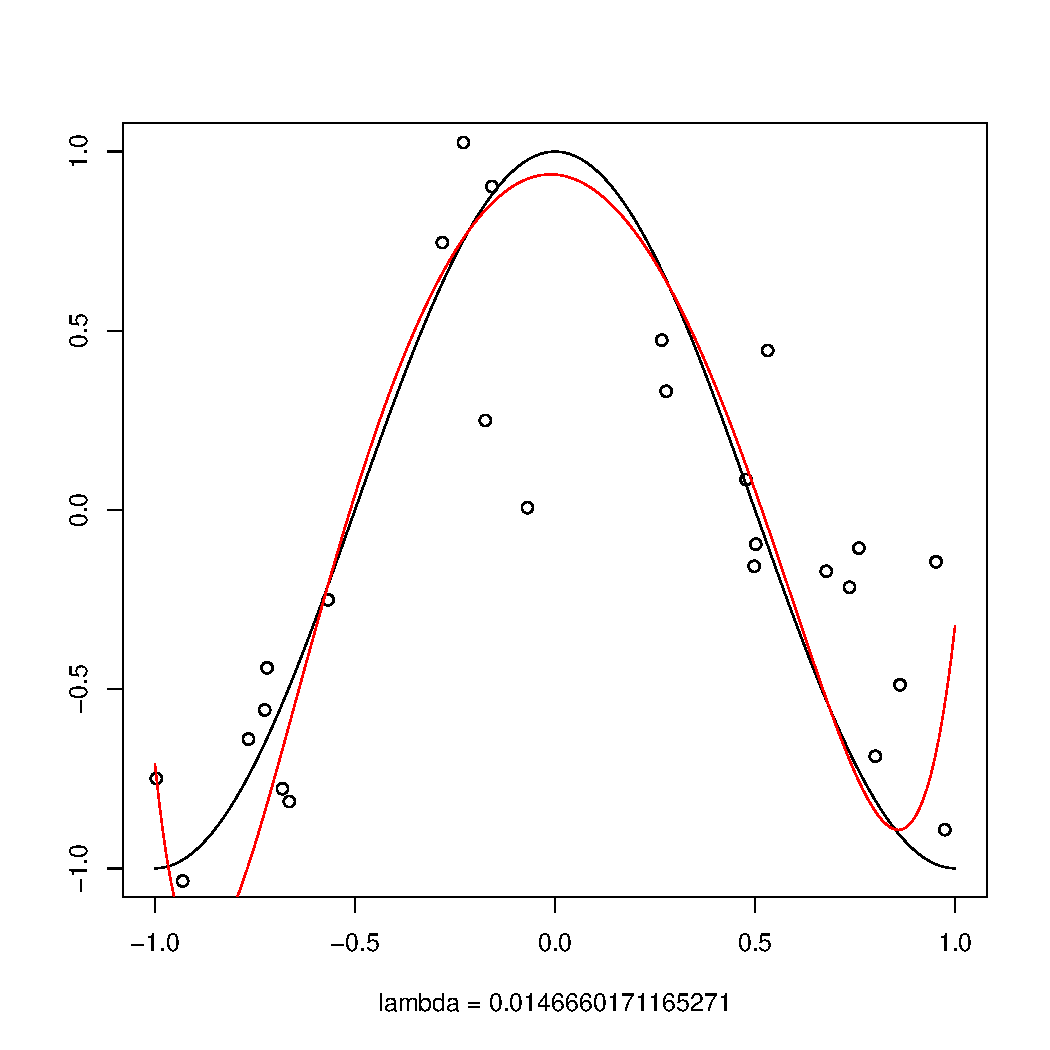
\includegraphics[trim={0em 1em 0em 3.4em}, clip]{cvbest.pdf}}
    \caption{\label{f:cvbest} Fitted polynomial, $\lambda \approx 0.015$}
   \end{center}
    \end{figure}


\end{frame}
    
    




\end{document}

